\documentclass[a4paper,oneside,12pt]{article}

\usepackage[english, francais]{babel}
\usepackage[utf8]{inputenc}  
\usepackage[T1]{fontenc}       
\usepackage{color}
\usepackage{fancyhdr}
\usepackage{lastpage}
\usepackage{graphicx} 
\usepackage{makeidx}
\usepackage{amsmath}


\usepackage{xspace}
\usepackage{picins}

\usepackage{tikz}

\newcommand{\fig}[3]{
  \begin{figure}[h]
    \begin{center}
      \includegraphics[width=0.8\linewidth]{#1}
      \caption{#2}
      \label{#3}
    \end{center}
  \end{figure}
}

\newcommand{\smallfig}[4]{
  \begin{figure}[h]
    \begin{center}
      \includegraphics[width=#1\linewidth]{#2}
      \caption{#3}
      \label{#4}
    \end{center}
  \end{figure}
}

\newcommand{\leo}{L\'eo B\textsc{audouin}\xspace}
\newcommand{\rory}{Rory F\textsc{lemmer}\xspace}
\newcommand{\chedli}{Chedli B\textsc{ouzgarrou}\xspace}
\newcommand{\umassey}{universit\'e de Massey\xspace}

\newcommand{\eme}[1]{$#1^{\grave{e}me}$}
\newcommand{\ere}[1]{$#1^{\grave{e}re}$}
\newcommand{\er}[1]{$#1^{er}$}

\newcommand{\logo}{images/logo-IFMA.jpg}

\newcommand{\titre}{Force control of anthropomorphic arm}
\newcommand{\auteur}{\leo}
\newcommand{\pole}{MMS -- M\'ecatronique}
\newcommand{\file}{lbaudouin-universite.pdf}
\newcommand{\resumeFR}{Ce rapport est un compte rendu du stage en universit\'e r\'ealis\'e dans le cadre de l'Ann\'ee Internationale. Il expose la partie technique concernant le travail effectu\'e sur le th\`eme 'Controle en force d'un bras anthropomorphe'.}
\newcommand{\resumeEN}{This report summarize the university internship during my year abroad.
It sets out the technical work on the theme 'Force control of anthropomorphic arm'}
\newcommand{\motsclefsFR}{Stage universit\'e, Massey University, robotique, m\'ecatronique}
\newcommand{\motsclefsEN}{University internship, Massey University, robotics, mechatronics}

\newcommand{\saut}{\vspace{5mm}}

%\setlength{\topmargin}{-1.cm}  
\setlength{\textheight}{23.5cm}    
\setlength{\oddsidemargin}{0.cm}
\setlength{\evensidemargin}{0.cm}
\setlength{\textwidth}{16.cm}

\begin{document}

\thispagestyle{empty}
\textcolor{blue}{Ministère de l'Enseignement Supérieur et de la Recherche}\\
\vspace{5mm}
\begin{centering}

  \includegraphics[width=3.0cm]{\logo} ~
  
\includegraphics[width=7.0cm]{images/logo-massey-university}

\end{centering}

\vspace{5mm}
\begin{center} 
\begin{large}
\textbf{Rapport de Stage en Universit\'e}
\end{large}
\\\vspace{3mm}--\vspace{3mm}\\
\begin{Huge}
\textbf{\titre}
\end{Huge}
\\
\vspace{10mm}
\begin{LARGE}
\leo\\

\vspace{5mm}
\eme{3} \textit{année -- P\^ole MMS -- Mécatronique}\\
\end{LARGE}
\vspace{5mm}
\today
\end{center}
%\vspace{5mm}

\begin{flushright}
\begin{large}
Universit\'e :\\

%\vspace{2mm}
\textbf{Massey University, New Zealand}\\

\vspace{3mm}
Tuteur Universit\'e :\\

%\vspace{2mm}
\textbf{\rory}\\

\vspace{3mm}
Tuteur IFMA :\\

%\vspace{4mm}
\textbf{\chedli}\\

\vspace{3mm}
Date : du 01 septembre 2011 au 10 janvier 2012
\end{large}
\end{flushright}

\vspace{5mm}
\begin{flushright}
Massey University,
\begin{footnotesize}
Tennent Drive\\
Palmerston North,
4474,
New Zealand\\
\end{footnotesize}
\vspace{2mm}

\textcolor{red}{I\textsc{nstitut} F\textsc{ran\c{c}ais de} M\textsc{\'ecanique} A\textsc{vanc\'ee}}\\
\begin{footnotesize}
\textcolor{blue}{C\textsc{ampus de} C\textsc{lermont}-F\textsc{errand} - L\textsc{es} C\textsc{\'ezeaux} - \textsc{bp} 265\\
63175 A\textsc{ubi\`ere} C\textsc{edex} - F\textsc{rance}}\\
\textcolor{blue}{T\textsc{el}. +33 (0)4 73 28 80 00 - F\textsc{ax} +33 (0)4 73 28 81 00\\
leo.baudouin@ifma.fr -} \textcolor{red}{www.ifma.fr}\\
\end{footnotesize}
\end{flushright}

\newpage
\setlength{\topmargin}{-1.cm}  

\thispagestyle{empty}

%\addcontentsline{toc}{section}{\numberline{}Identification}

\noindent \textcolor{blue}{Minist\`ere de l'Enseignement Sup\'erieur et de la Recherche}

\begin{flushright}
\vspace*{-0.80cm}
\includegraphics [width=3.0cm]{\logo}
\end{flushright}
\vspace{-1cm}
%%% Fin En-t�te
%----------------------------------------------------------------------------------------
%%% Premier cadre : Identification
\vfill
\rule[6pt]{16cm}{1pt}
\large{TITRE DU RAPPORT : \\
\textbf {\titre}
\newline
\large{\hfill \title \\}
\rule[6pt]{16cm}{.5pt}
\large{AUTEUR(S) :  {\auteur \hfill \pole}\\}
\rule[0pt]{16cm}{.5pt}
\begin{center}
\begin{tabular}{ccc}
Date du document & Nb pages & R\'ef\'erence du document \\ 
\today & \pageref{LastPage} & \file  %
\end{tabular}
\end{center}
\rule[6pt]{16cm}{1pt}
%----------------------------------------------------------------------------------------
\vfill
\noindent \rule[0pt]{16cm}{1pt}
\large{R\'ESUM\'E :} \\ \normalsize {\resumeFR} \\
\rule[0pt]{16cm}{.5pt}
\large{Mots-cl\'e : \motsclefsFR \\}
\rule[0pt]{16cm}{1pt}
%----------------------------------------------------------------------------------------
\selectlanguage{english}
\vfill
\label{English}
\noindent\rule[0pt]{16cm}{1pt}
\large{ABSTRACT:} \\ \normalsize {\resumeEN} \\
\rule[0pt]{16cm}{.5pt}
\large{KeyWords: \motsclefsEN \\}
\rule[0pt]{16cm}{1pt}
%----------------------------------------------------------------------------------------
\selectlanguage{francais}%
\vfill

\setlength{\topmargin}{0.cm}

\newpage
\pagestyle{empty}

\fancyhf{}
\fancyhead[L]{Rapport de Stage en Universit\'e}
\fancyfoot[R]{\thepage/\pageref{LastPage}}
\fancyfoot[L]{\leo~-~ \eme{3} \textit{année MMS - Mécatronique}}

%Table of contents

\pagestyle{fancy}
\tableofcontents
\addtocontents{toc}{\protect\thispagestyle{fancy}}
\addtocontents{toc}{\protect\pagestyle{fancy}}

\newpage

\section*{Avant Propos}
\addcontentsline{toc}{section}{\numberline{}Avant-propos}

Je tiens tout d'abords à remercier l'IFMA d'avoir accepté que le début de ma thèse soit compté comme mon stage de fin d'étude.
Effectivement suite à un master, réalisé en parallèle des enseignements de l'IFMA, j'ai souhaité poursuivre dans la recherche au travers d'un doctorat.

\'Etant donné que les premiers mois d'une thèse sont principalement destinés à faire un étude de l'état de l'art dans le domaine concerné, ce rapport contiendra un nombre important de citations d'articles scientifiques. Il ne sera donc pas exactement comme un rapport de PIFE traditionnel.

Ayant effectué plusieurs stages dans la robotique mobile et avec un master en Imagerie \& Vision en poche, j'ai décidé de travailler sur un sujet cumulant ces deux aspects scientifiques.

Je remercie \tuteur, mon tuteur de thèse, de m'avoir accepté dans son équipe de recherche. Je remercie également Omar \textsc{Ait-Ader} et Jonathan \textsc{Courbon} pour l'aide qu'ils m'ont apporté.
\newpage

\section{Introduction}

Avec les GPS, les radars de recul, les assistants de créneaux et autres gadgets, les aides à la conduite deviennent de plus en plus intelligentes.
Devant le nombre de capteurs et de calculateurs embarqués on est en droit de se demander si le conducteur humain dans une voiture est encore nécessaire.

Il existe déjà des projets comme la voiture Google qui roule de façon autonome sur certaines les routes américaines. Mais ces voitures nécessite un nombre très important de capteurs avec une précision très importante.
On y retrouve un GPS précis au centimètre, des télémètres lasers plans ou 3D, ainsi que des accéléromètres multi-directionnels.

Ces capteurs ont un coût important et ne sont pas à la porté des particuliers.
C'est pourquoi nous travaillons sur des véhicules autonome utilisant la vision, le prix d'une caméra étant largement inférieur à celui d'un télémètre laser 3D.

Cependant, les algorithmes en développement ne sont pas encore adaptés à des véhicules roulant à haute vitesse.
En attendant que le matériel et les programmes le permettent, nous allons utiliser un véhicule autonome roulant à basse vitesse, un VipaLab (voir figure~\ref{fig:vipalab}).

\fig{images/videH.jpg}{Un VipaLab, véhicule de la société \warning{APOJEE}}{fig:vipalab}

Le but final est d'avoir une flotte de véhicules autonomes, en libre service, dans le centre ville de Clermont-Ferrand.
A partir d'un point initial, le robot devra être capable de planifier son trajet jusqu'à la destination souhaitée par l'utilise et de l'exécuter de manière totalement autonome mais sécurisé.
Effectivement le robot pourra être amené à rouler dans des zones piétonnes (respect des piétons, évitement de collisions) mais également sur certaines portions de route (respect du code de la route).

Dans un environnement aussi contraint qu'une zone piétonne, le robot doit pouvoir observer ce qu'il se passe tout autour de lui.
L'utilisation de caméras perspectives avant et arrière ne sera pas obligatoirement suffisant dans certains cas.
C'est pourquoi nous avons souhaité travailler avec des caméras omnidirectionnelles (caméra catadioptrique, voir figure~\ref{fig:camcata}).

\smallfig{0.4}{images/videV}{Caméra omnidirectionnelle composée d'une caméra affine et d'un miroir parabolique}{fig:camcata}

Notre flotte de véhicule ne sera pas obligatoirement homogène, on y retrouvera différents robots (véhicules) et différents capteurs (caméras).
La différences entre les robots n'impactera pas sur notre travaille car la gestion de la trajectoire sera calculé par un programme tiers.
La différences entre les caméras aura, quand à elle, un impacte très important sur les travaux à réalisés.
Il existe de nombreux algorithme de SLAM\footnote{Simultaneous Localisation And Mapping -- Cartographie et localisation simultanée} utilisant la vision.
Cependant ils ne se concentrent que sur un type de caméra à la fois.

L'innovation demandé dans ce travail de recherche est de mettre en place de nouveaux algorithmes permettant la cartographie et la navigation pour une flotte de robots munies de caméras de type différents.
Pour parler une paire de caméras, composée d'une caméra perspective et d'une caméra omnidirectionnelle, nous utiliserons le terme de paire hybride, d'où la notion de vision hybride.

\newpage

\section{État de l'art}

\subsection{Vision, Reconstruction 3D}

\subsubsection{Vision classique}

Nos robots seront équipés de caméras de types différents, On va donc commencer par traiter au cas par cas les algorithmes nécessaires pour les caméras.
La caméra la plus courante est la caméra perspective (ou \textit{pinhole} en anglais).
De très nombreux ouvrages existent sur la reconstruction à l'aide d'une caméra perspective, on retrouve notamment  \citetitle{Hartley03Book} de \citeauthor{Hartley03Book} \cite{Hartley03Book}.

A partir d'images successives issues d'un même capteur, nous pouvons reconstruire un modèle 3D de l'environnement parcouru par un humain ou un robot mobile.
La reconstruction se fait sous la forme d'un nuage de points plus ou moins compact en fonction des détails présents dans les images.
Une fois un nuage de points obtenu, nous pouvons affiner ce modèle en effectuant un ajustement de faisceaux (\textit{bundle adjustement}), cette opération consiste à passer un Levenberg-Marquardt\footnote{Algorithme interpolant l'algorithme de Gauss-Newton et l'algorithme de la descente de gradient} sur les données afin de minimiser les erreurs de projection.

On retrouve également les techniques de reconstruction avec deux caméras dans le livre \cite{HoraudBook}, \citetitle{HoraudBook} de \citeauthor{HoraudBook}.

\warning{Cependant une dérive apparaît ...}


\subsubsection{Vision mixte}

L'utilisation complémentaire de caméras omnidirectionnelles, nous pouvons nous demander si nous pouvons utiliser les deux types de caméras simultanément afin de créer le nuage de point.
On retrouve ce genre de travaux quand les travaux de
\citeauthor{Sturm02}, \citetitle{Sturm02} \cite{Sturm02}.
Certains problèmes restent cependant à éclaircir, comme la calibration des caméras omnidirectionnelles.

En lisant ce papier, on se demande alors comment extraire les variables intéressantes comme la matrice essentielle ou les matrices de rotation et de translation.

Une autre question consiste à trouvé un moyen de trouver des points correspondants entre les images perspectives et les images omnidirectionnelles.
Le papier \cite{Puig08} utilise les descripteurs SIFT\footnote{Scale Invariant Feature Transform}.
Il construit ensuite une matrice fondamentale à l'aide des correspondances.
On retrouve des matrices $\mathbf{F}_{43}$, $\mathbf{F}_{63}$ and $\mathbf{F}_{66}$.
On retrouve le même problème que pour le papier précédent pour avoir les matrices importantes \textbf{R} et \textbf{t} ou \textbf{E} depuis $\mathbf{F}_{xx}$?

\newpage

\begin{minipage}[c]{0.5\textwidth}
  \centering
  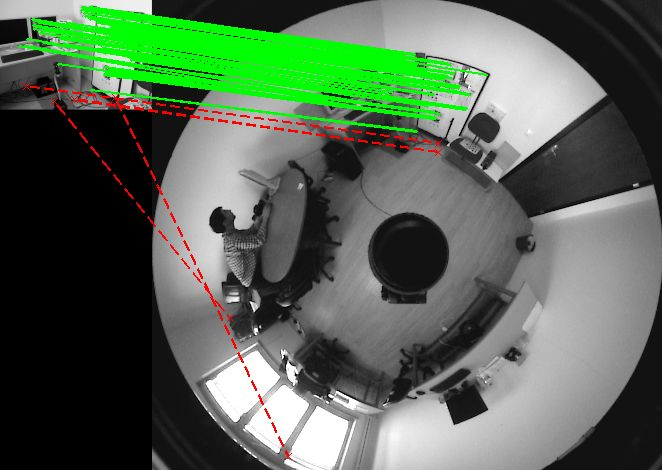
\includegraphics[width=3.0in]{images/Bastanlar09.png}
  \captionof{figure}{Caption for image}
  \label{fig:sample_figure}
\end{minipage}
\begin{minipage}[c]{0.5\textwidth}


  %\begin{tabular}{l l}
  %\begin{minipage}{0.5\linewidth} 
  %\smallfig{0.5}{images/Bastanlar09.png}{[Bastanlar09PhD] Structure from Motion for Systems with Perspective and Omnidirectional Cameras}{fig:bastanlar}
  %\end{minipage}  
  %&
  %\begin{minipage}{0.5\linewidth}
  SfM with hybrid system [Bastanlar09PhD] Structure from Motion for Systems with Perspective and Omnidirectional Cameras\\
  Compute 3D reconstruction with hybrid pair of cameras.\\
  $$q_p^t K_p^{-t} ~E~ \theta^t \hat{K}_c^t \hat{q}_c = 0$$\\
  $\Rightarrow$ No information on calibration of omnidirectional camera $\hat{K}_c$ (see Puig PhD page 25)
  %No information on \textbf{E} computation and \textbf{R},\textbf{t} extraction.
\end{minipage}
%\end{tabular}

%\begin{tabular}{l l}
\smallfig{0.5}{images/Goedeme07.png}{[Goedemé07] Omnidirectional Vision based Topological Navigation}{fig:goedeme}
%&
%\begin{minipage}{0.5\linewidth}

Lorsqu'on a une image, classique ou omnidirectionnelle, nous pouvons nous demander ce que nous devons voir sur cette image.
Quelles sont les amères intéressantes, et pourquoi ?

On retrouve généralement :
\begin{itemize}
\item Le point
\item La droite
\item La courbe
\item L'ellipse ou cercle
\end{itemize}
Chaque type d'amère possède des avantages et des inconvénients :
\begin{table}[h]
  \begin{center}
    \begin{tabular}{|c|c|c|}
      \hline
      Type & Avantages & Inconvénients \\
      \hline
      Point & Générique & Comparaison \\
      Droite & Robuste & Peu présent en extérieur \\
      Courbe & Plus de liberté & Sensible aux rotations \\
      Ellipse & Facile à sélectionner & Peu présent en général\\
      \hline
    \end{tabular}    		
  \end{center}
  \caption{Comparaison des amères}
\end{table}

Nous ne pourrons donc pas utiliser les courbes et les ellipses car pour l'un il nous sera difficile de les définir, et pour l'autre on ne les retrouve pas en assez grand nombre dans un environnement classique.
Les lignes sont particulièrement présentes dans les environnements intérieurs, mais malheureusement beaucoup moins en extérieur.
Notre robots devant naviguer principalement en extérieur, ce type d'amère est incompatible avec notre besoin.
Il reste donc les points, qui sont naturellement présent dans toutes les images nettes d'un environnement.
Le défi sera donc de caractériser les différents points de l'image afin de pouvoir les comparer et les appairer.
Plusieurs outils sont à notre disposition, il s'agit de descripteurs.
On va caractériser une imagette d'une taille fixe autour du point, puis enregistrer l'information en même temps que la position du point dans l'image.

%\end{minipage}
%\end{tabular}
\warning{Répétition}

Dans le cas des images omnidirectionnelles, compte tenu de la déformation des images, les seules amères pouvant être utilisées sont :
\begin{itemize}
\item Les points : les appariements se font avec principalement SIFT
\item Les droites : détection de droites verticales (droites se coupant au centre de l'image), droites parallèles (sous forme de coniques dans l'image)
\end{itemize}



\smallfig{0.2}{images/Dame10.png}{[Dame10PhD] A unified direct approach for visual servoing and visual tracking using mutual information}{fig:dame}
Dame \cite{Dame10PhD} propose un moyen de comparaison de deux imagettes plus performant que les algorithmes proposés : SSD\footnote{Sum of Squared Differences} or ZNCC\footnote{Zero-mean Normalized\\Cross Correlation}.
Comparer MI avec SIFT, SURF et autres descripteurs lors des cas de vision hybride perspective/catadioptrique.  

\subsubsection{Trajectoire}

En reconstruisant le modèle 3D de l’environnement, on obtient également le chemin parcouru lors de la prise des images.
Ce résultat est moins précis qu'avec un GPS car la fréquence d'acquisition des images est généralement plus élevée.

\smallfig{0.2}{images/Rituerto10.png} {Ici la courbe noire est la trajectoire réelle, la bleue est obtenue par l'odométrie, la rouge par la vision omnidirectionnelle} {fig:rituerto}
Dans le papier \cite{Rituerto10}, l'auteur propose l'utilisation du filtre de Kalman (EKF\footnote{Extended KalmanFilter}) avec une caméra omnidirectionnelle. On remarque également l'utilisation de SIFT pour les mises en correspondances dans le cas d'images omnidirectionnelles. Ses résultats montrent qu'il obtient une meilleur précision qu'avec un SLAM classique. 


\subsection{Fusion de cartes}

Chacun des robots va créer sa propre carte basée sur les informations visuelles acquises lors de son déplacement.
Lorsque qu'un autre robot va croiser la trajectoire parcourue par le premier, il y aura des informations identiques dans les deux cartes, il serait donc important de fusionner les informations dans une seule carte plus globale.

On retrouve un grand nombre de travaux pour la robotique mobile dans le cas de robots embarquant un capteur de type laser.

\smallfig{0.2}{images/Konolige03.png}{[Konolige03] Map Merging for Distributed Robot Navigation}{fig:konolige}
Basé sur une méthode de vraisemblance (\textit{likehood}), Konolige \cite{Konolige03} permet de re-situer une sous-partie de carte au sein d'une carte globale ayant un a-priori sur la position.\\
$\Rightarrow$ Utilisation de carte dense telle qu'une cartographie laser.




\smallfig{0.2}{images/Gutmann99.png}{[Gutmann99] Incremental Mapping of Large Cycle Environments}{fig:gutmann}
Le papier \cite{Gutmann99} parle de la recherche de recouvrement de scan dans une démarche d'exploration d'environnement. 
Il utilise des parties de la carte globale afin de voir si le motif se retrouve autre part dans la carte pour effectuer une fermeture de boucle.\\
$\Rightarrow$ Utilisation de carte dense telle qu'une cartographie laser.



\smallfig{0.2}{images/Strasdat10.png}{[Strasdat10] Scale Drift-Aware Large Scale Monocular SLAM}{fig:strasdat}   
Un des papiers les plus intéressant en vision monoculaire est \cite{Strasdat10}, qui, à l'aide d'une caméra perspective reconstruit un batiment en utilisant un ajustement de faisceaux qui corrige la dérive du facteur d'échelle.
Un pré-ajustement est effectué avec une fenêtre glissante (quelques images), puis une fois la fermeture de boucle détectée, un ajustement global sur 7 degrés de liberté (rotation, translation échelle) est effectué. 



\smallfig{0.2}{images/Korrapati11.png}{[Korrapati11] Efficient Topological Mapping with Image Sequence Partitionning}{fig:korrapati}  
Pour les expériences avec une caméra omnidirectionnelle \cite{Korrapati11}, un système de gestion des amères à été mis en place afin de pouvoir retrouver rapidement les fermetures de boucle.\\
Ce système pourra être utilisé dans le cas de notre étude (voir SoViN, \ref{subsub:sovin}).



\subsection{Multi-robots}

Comme annoncé précédemment, notre étude portera sur une flotte de robots mobiles.
Il y a donc un aspect supplémentaire à prendre en compte, la coopération.

\smallfig{0.2}{images/Hukui10.png}{[Hukui10] Mutual Localization of Sensor Node Robots}{fig:hukui}  
Le papier \cite{Hukui10} se base sur l'utilisation des connaissances sur les positions relatives des robots afin d'améliorer la qualité de la localisation globale.
Si un robot connaît la position d'un autre robot par rapport à sa position courante, il peut utiliser les informations acquises par le second pour alimenter sa base de données.

Quelques points importants restent à éclaircir comme comment localiser les robots entre eux ?
Effectivement, nous devons faire la différence entre un VipaLab et une voiture classique sus une image omnidirectionnelle, c'est donc un problème de détection puis de suivi d'objets.
L'autre point est la précision de position (et d'orientation) relative des robots obtenue par la vision.



\smallfig{0.2}{images/Howard06.png}{[Howard06] Multi-robot Simultaneous Localiszation and Mapping using Particule Filters}{fig:howard}  
\warning{J'ai pas bien compris} le papier \cite{Howard06}


\smallfig{0.4}{images/Aragues11.png}{[Aragues11PhD] Distributed Algorithms on Robotic Nectwoks for Coordination in Perception Tasks}{fig:aragues}  
La thèse de \citeauthor{Aragues11PhD} \cite{Aragues11PhD} montre comment mettre en place un système efficace de communication inter-robots dans le cadre de fusion de cartes.
Map merging with multi robots, one camera type. Use SIFT/SURF and 3D points.\\
$\Rightarrow$ Improve with mutli-camera sensors. 



\subsection{SoViN}
\label{subsub:sovin}

       
La librairie \emph{SoViN}\footnote{Software for Visual Navigation} développée par J. \textsc{Courbon}\footnote{En collaboration avec L. \textsc{Lequièvre}, Y. \textsc{Mezouar} et E. \textsc{Royer}} permet une gestion optimisée des bases de données dans le cadre de la vision pour robot mobile.
L'architecture proposée permet d'enregistrer simultanément une image, les points 2D extraits avec leur descripteurs respectifs, les points 3D reconstruits ainsi que la position du robot si elle est connue.

Pour pouvoir l'utiliser dans le cadre de ma thèse il faut donc ajouter/revoir les blocks suivants :
\begin{itemize}
\item Multi-robots, gérer l'utilisation de plusieurs sources d'images
\item Carte globale, résultat de la fusion de cartes locales
\item Fermeture de boucles, pour détecter des redondances d'informations entre robots
\item Information mutuelle, comme nouveau type de descripteur
\end{itemize}

\smallfig{0.7}{images/sovin.png}{Interface du logiciel \emph{SoViN} par J. \textsc{Courbon}}{fig:SOVIN}

Une interface graphique est proposée pour construire et visualiser la base de donnée.
Le fonctionnement détaillé est visible dans \cite{Lequievre08}, qui mentionne \warning{A LIRE}.

\newpage

\section{Vision}

Cette partie sera une consacrée à la partie théorique de la reconstruction 3D.
Dans un premier temps nous verrons le cas de la reconstruction à partir d'une paire de caméras classiques.
Nous verrons ensuite le modèle unifié pour les caméras catadioptrique.
Nous aborderons au final la vision hybride.

\subsection{Reconstruction 3D}
\label{sub:reconstruction}

La reconstruction 3D à partir de deux vues perspectives a été très bien formalisé dans le livre de \citeauthor{Hartley03Book} \cite{Hartley03Book}.
En prenant deux vues d'une même caméra perspective, nous devons calculer le déplacement entre les lieux de prise de vue.
Celui ci est déterminé par une matrice de projection $\mathbf{P}$ qui se compose de deux matrices $\mathbf{R}$ et $\mathbf{t}$, respectivement la matrice de rotation et la matrice de translation.

La projection d'un point $\mathbf{X}$ dans l'espace donne le point $\mathbf{m}$ dans le plan image :
\begin{equation}
s \underbrace{\begin{pmatrix}u \\ v \\ 1\end{pmatrix}}_{\mathbf{m}} = 
\underbrace{\begin{pmatrix}f_u && 0 && u_0 \\ 0 && f_v && v_0 \\ 0 && 0 && 1\end{pmatrix}}_{\mathbf{K}} . 
\underbrace{\begin{pmatrix}r11 && r12 && r13 && t1 \\ r21 && r22 && r23 && t2 \\ r31 && r32 && r33 && t3\end{pmatrix}}_{[\mathbf{R~t}]} . 
\underbrace{\begin{pmatrix}X \\ Y \\ Z \\ 1\end{pmatrix}}_{\mathbf{X}} 
\end{equation}

\begin{equation}
s.\mathbf{m} = \mathbf{K}.\mathbf{P}.\mathbf{X}
\end{equation}
Avec : 
\begin{itemize}
\item $\mathbf{m}$ le point dans l'image
\item $\mathbf{P}$ la matrice de projection 
$\mathbf{P} = [ \mathbf{R} ~ \mathbf{t} ]$
\item $\mathbf{K}$ la matrice des paramètres intrinsèques (calibration)
\item $s$ est un facteur réel quelconque ($s \in \Re$)
\end{itemize}

\subsubsection{Calibration}
\label{subsub:calibration}
La calibration d'une caméra perspective est réalisé à partir d'une mire \cite{??}.

\subsubsection{Méthode}

Comme nous avons pu voir précédemment, les seuls informations que l'on va utiliser dans les images sont des points.
Pour donner un sens à ces listes de points, ils seront appairés.
C'est à dire que chaque point dans la première image devra avoir un point correspondant dans la seconde.

On va pouvoir calculer un matrice regroupant toutes les informations possible de tiré de cette configuration.
Cette matrice ce nommera la matrice fondamentale, notée $\mathbf{F}$.
Elle est définit pour toutes paires de points $i$ dans les images 1 et 2, par la suite l'indice $i$ sera omis.
\begin{equation}
\mathbf{m}_{i,1}.\mathbf{F}.\mathbf{m}_{i,2} = 0
\label{eq:fondamentale}
\end{equation}
Connaissant la matrice intrinsèque de la caméra (voir \ref{subsub:calibration}), nous pouvons éliminer les facteurs induit par les focales, afin de normaliser la matrice fondamentale.
On obtiendra la matrice essentielle $\mathbf{E}$ :
\begin{equation}
\mathbf{E} = \mathbf{K}_1^{T} . \mathbf{F} . \mathbf{K}_2
\end{equation}
Si les deux images sont acquis par la même caméra, on aura $\mathbf{K}_1 = \mathbf{K}_2$.

Nous pouvons obtenir la matrice essentielle directement depuis la liste de points, en normalisant les points eux-même.
\begin{equation}
(\mathbf{m}_{i,1}.\mathbf{K}_1^{-T}).\mathbf{E}.(\mathbf{K}_2^{-1}.\mathbf{m}_{i,2}) = 0
\label{eq:essentielle}
\end{equation}


Afin d'obtenir les matrices $\mathbf{R}$ et $\mathbf{t}$, nous devons utiliser une autre formulation de $\mathbf{E}$ :
\begin{equation}
\mathbf{E} = \mathbf{R} . [\mathbf{t}]_x
\end{equation}
Avec $[\mathbf{t}]_x$ la matrice anti-symétrique\footnote{Si $\mathbf{t}=\begin{pmatrix}t_1\\t_2\\t_3\end{pmatrix}$, alors $[\mathbf{t}]_x=\begin{pmatrix}0&-t_3&t_2\\t_3&0&-t_1\\-t_2&t_1&0\end{pmatrix}$} du vecteur $\mathbf{t}$.

Nous pouvons maintenant extraire $\mathbf{R}$ et $\mathbf{t}$. Pour celà nous devons décomposer la matrice essentielle :
$$\mathbf{E}=\mathbf{U} \mathbf{\Sigma} \mathbf{V}^T$$
Nous avons, $ \mathbf{\Sigma} = \begin{pmatrix}s&0&0\\0&s&0\\0&0&0\end{pmatrix}$, alors:
\begin{equation}
[\mathbf{t}]_x = \mathbf{V} \mathbf{W} \mathbf{\Sigma} \mathbf{V}^T
\end{equation}
\begin{equation}
\mathbf{R} = \mathbf{U} \mathbf{W}^{-1} \mathbf{V}^T
\end{equation}
Avec, $\mathbf{W}=\begin{pmatrix}0&1&0\\-1&0&0\\0&0&1\end{pmatrix}$




\subsection{Modèle unifié}

Pour les caméras catadioptriques, un modèle permettant de représenter les caméeas munies d'un mirroir plan, parabolique, hyperbolique, elliptique a été mis en place.

Ce modèle unifié, appelé modèle sphérique, prends en entré un seul paramètre $\xi$ pour représenter le mirroir.

\fig{images/videH}{Modèle sphérique pour caméras catadioptriques}{fig:modeleunifie}

\subsubsection{Modèle de projection}

Soit $\mathbf{X}$ un point dans le repère monde.
On suppose la caméra au point $O$ de coordonnées $(0,0,0)$ avec l'axe $\vec{z}$, l'axe principal de la caméra.

On va projeter le point $X$ sur la sphère unitaire centrer en $O$. On obtiendra le point $X_m$.
\begin{equation}
X_m = \frac{X}{\rho}
\end{equation}
Avec $\rho = ||X|| = \sqrt{X^2+Y^2+Z^2}$.

On projete enfin le point $X_m$ sur le plan de $Z = 1 - \xi$ :
\begin{equation}
x = \begin{bmatrix}  \frac{X}{Z+\xi \rho} && \frac{Y}{Z +\xi \rho} && 1 \end{bmatrix}^{T}
\end{equation}

Pour finir on applique la transformée homographique due aux paramètres intrinsèques de la caméra, pour obtenir le point $m$ dans l'image.
\begin{equation}
m= K x
\end{equation}

\subsubsection{Retroprojection}

A partir du point $m$ dans l'image on souhaite avoir le point 3D dans le repère monde correspondant.

\begin{equation}
x = \begin{bmatrix} x && y && 1 \end{bmatrix}^{T} = K^{-1} m
\end{equation}

On inverse la fonction de projection pour obtenir les coordonnées du point du la shpère :
\begin{equation}
X_m = (\nu^{-1} + \xi) \bar{x}
\end{equation}
\begin{equation}
\bar{x} = \begin{bmatrix}x && y && \frac{1}{1+\xi \mu} \end{bmatrix}^{T}
\end{equation}
Avec :
\begin{equation}
  \left \{
  \begin{matrix}
    \mu = \frac{-\gamma-\xi(x^2+y^2)}{\xi(x^2+y^2)-1} \\
    \gamma = \sqrt{1+(1-\xi^2)(x^2+y^2)}
  \end{matrix}
 \right.
\end{equation}



\subsection{Vision Hybride}
Puig \cite{Puig08}

Pour les points de l'image catadioptrique, nous devons utilisé les coordonnées \cite{lifted}:
$$\hat{\mathbf{q}}=\begin{pmatrix}q_1^2+q_2^2\\q_1q_2\\q_2q_3\\q_3^2\end{pmatrix}$$
Nous avons :
\begin{equation}
\hat{\mathbf{q}}_c^T\mathbf{F}_{cp}\mathbf{q}_p=0
\end{equation}
On défini $\mathbf{B}_c$ ($3\times4$ matrice) pour représenter la matrice de projection pour la caméra catadioptrique.
La matrice essentielle ne peut pas \^etre calculé comme dans la section~\ref{sub:reconstruction} car $\mathbf{B}_c$ n'est pas une matrice de rotation :
\begin{equation}
\mathbf{E} \neq \mathbf{B}_c^T \mathbf{F}_{cp} \mathbf{K}_p
\end{equation}

\newpage

\section{Stratégie}
\label{sec:strategie}

\subsection{Carte locale}

Afin de pouvoir se déplacer en autonomie, chaque robot aura une carte locale associée aux déplacements réalisés pendant la séquence de cartographie.
Sur cette période, les robots sont dirigés manuellement afin de parcourir les lieux qui serviront lors de la phase de navigation autonome.

Les cartes locales sont constituées des éléments repérables et calculables par le robots.
On retrouve donc :
\begin{itemize}
\item Les points d'intérêts dans l'image ainsi que leurs descripteurs associés
\item Les points 3D reconstruits
\item La trajectoire du robot calculée
\item Informations provenant d'autres capteurs comme l'odométrie
\end{itemize}

Les points d'intérêts sont extraits à l'aide de la méthode de Harris~\cite{Harris88}. Ce sont les points qui sont généralement situés aux intersections de segments ou qui ceux possèdent un contraste élevé avec ses voisins.
Un descripteur du point lui est associé, on utilisera dans un premier temps les descripteurs SIFT~\cite{Lowe99}, qui est insensible aux changement d'échelle et aux rotations.
D'autres types de descripteurs seront testé pour comparer les performances, comme les informations mutuelles, MSER, Ogre, SURF et si aucun n'est très performant pour le cas hybride, nous serrons dans l'obligation de mettre au point un niveau type de descripteur.

Dans un second temps on pourra envisager l'exploration autonome, c'est à dire que le robot générera lui même une trajectoire d'exploration afin d'alimenter sa collection d'images.

\subsection{Carte globale}

La carte globale est la fusion de toute les cartes locales.
Elle est construite par fusion itérative de deux cartes locales sécantes.

Dans un premier temps, un ordinateur central récupère toutes les cartes locales des différents robots.
La stratégie utilisée pour la fusion est la suivante :
\begin{enumerate}
\item A partir de deux nuages de points 3D, on cherche les correspondances 3D/3D, c'est-à-dire comment doit être déplacer le deuxième nuage de points 3D pour se superposé au mieux avec le premier.
Plusieurs solutions pourront être retournés.
\item Afin de rejeté les mauvaises solutions, on testera si les points 3D mis en correspondances sont réellement les même en comparant leurs descripteurs respectifs.
\item si le nombre de points 3D en correspondance restant est suffisant, la fusion de carte peut avoir lieux.
On applique la transformation (rotation, translation, échelle) à la deuxième carte et on ajoute tous les points à la première.
\end{enumerate}

Si les cartes ne sont pas sécantes, le robot devra garder en mémoire deux cartes distinctes afin de pouvoir les fusionner lui même si lors d'un nouveau parcours si passe de l'une à l'autre.

Dans un second temps on pourra envisagé la fusion de carte \emph{en ligne} lorsque deux robots sont assez proches pour communiquer et qu'ils trouvent un ou plusieurs endroits communs dans leurs cartes locales.

\subsection{Navigation}

L'étape de navigation peut débuter sans carte dans un mode d'exploration de l'environnement.
Cependant en présence d'individu, il est recommandé que les cartes soient vérifiées par un superviseur.
La navigation ne peut donc s'effectuer qu'une fois les cartes locales crées, et une carte globale si possible.

Le but final étant de pouvoir se déplacer de façon autonome d'un point A à un point B.
C'est à dire que le robot est déjà passé, au moins une fois, par les chemins qui lui est possible d'exploiter.
Il faudra donc obligatoirement que les deux points de départ et d'arrivée appartiennent à l'espace observé lors de la création des cartes.

Afin de générer une trajectoire optimale, nous utiliserons des algorithme de navigation classique déjà exploités par un grand nombre de robot mobile.
On fera particulièrement attention au respect du code de la route et à la sécurité des piétons en zone urbaine.
Un effort sera également à réalisé afin d'éviter les collisions dans les environnements dynamiques.
Ces travaux seront réalisés dans la deuxième partie de ma thèse. 


\newpage

\section{Conclusion}

Malgré plus de 15000 lignes de code pour le début d'une bibliothèque écrite en C++ afin réaliser mes travaux, je n'ai pas encore réussi à obtenir de résultats concluants pour la création et fusion de cartes pour la robotique.

Cette bibliothèque permet actuellement de construire un nuage de points 3D à partir d'une vidéo issue d'une caméra perspective calibrée.
Le cas de la caméra catadioptrique n'est pas encore complètement opérationnel.
La convergence du recalage entre les points 3D et les points 2D de l'image, n'est pas garantie et rend donc des résultats qui peuvent être aléatoires.

Le projet s'étend sur trois années et devra au final permettre de contrôler une flotte de robots de façon autonome.
Les six premiers mois de cette thèse, représentant mon stage de fin d'études, ont principalement été consacrés à l'étude bibliographique du domaine concerné par la thèse : la robotique mobile autonome, la vision omnidirectionnelle et la fusion de carte.
En parallèle à cette étude, une partie développement d'outils de base à été réalisé comme mentionné précédemment.

J'ai développé ces outils à partir des cours théoriques que j'ai eu en master \emph{Image et Vision} mais également à partir de livre comme 
\citetitle{Hartley03Book} 
de 
\citeauthor{Hartley03Book} 
\cite{Hartley03Book} 
et d'articles comme
\citetitle{Puig08} 
de 
\citeauthor{Puig08} 
\cite{Puig08}.

J'aurais aimé pouvoir utiliser des bibliothèques ou programmes existants développés au sein du laboratoire ou dans d'autres laboratoires similaires mais je n'y ai pas encore eu accès.
De plus une grande partie des chercheurs utilisent des outils de prototypage tel Matlab, et donc peu de code performant en C++ sont partagés.
Donc même si les méthodes sont connues et utilisées dans le laboratoire, j'ai du les re-développer moi même afin d'avoir une bibliothèque adéquate, partagée avec la communauté de façon libre et gratuite.

Concernant la vitesse d'avancement du projet, je considère que beaucoup de temps a été utilisé pour l'étude bibliographique.
Une autre partie à pour l'instant été consacrée à la programmation d'outils afin d'acquérir les connaissances nécessaires pour la reconstruction 3D.
Il est donc normal que peu de résultats soient encore exploitables.

\newpage

%\bibliographystyle{plain}
%\bibliography{./main}
\newpage

%\appendix

\section{Publication Humanoids 2011}

Publication pour la conférence Humanoids 2011.\\
\emph{Real-time Replanning Using 3D Environment for Humanoid Robot}\\
\leo, \nicolas, \olivier, \thomas, \eiichi et \florent.




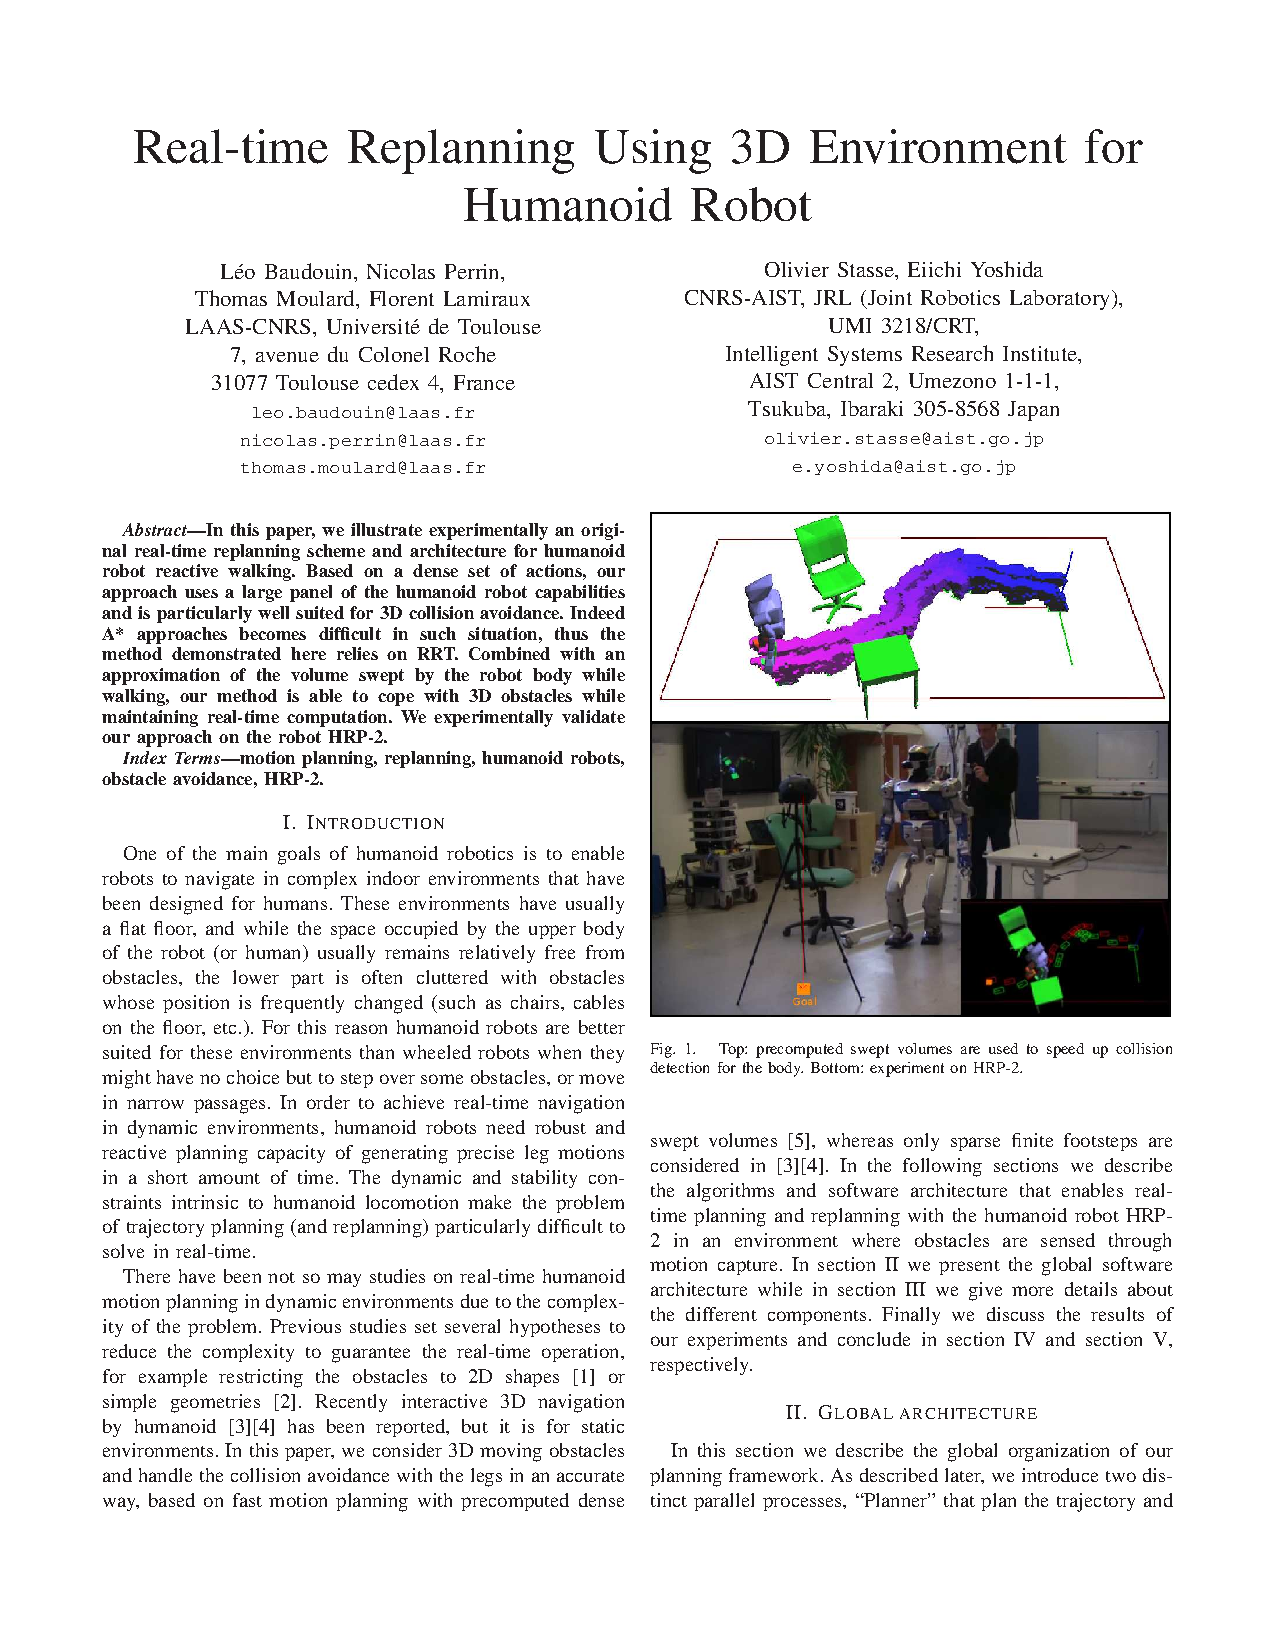
\includepdf[page=1]{humanoids11-lbaudouin.pdf} 
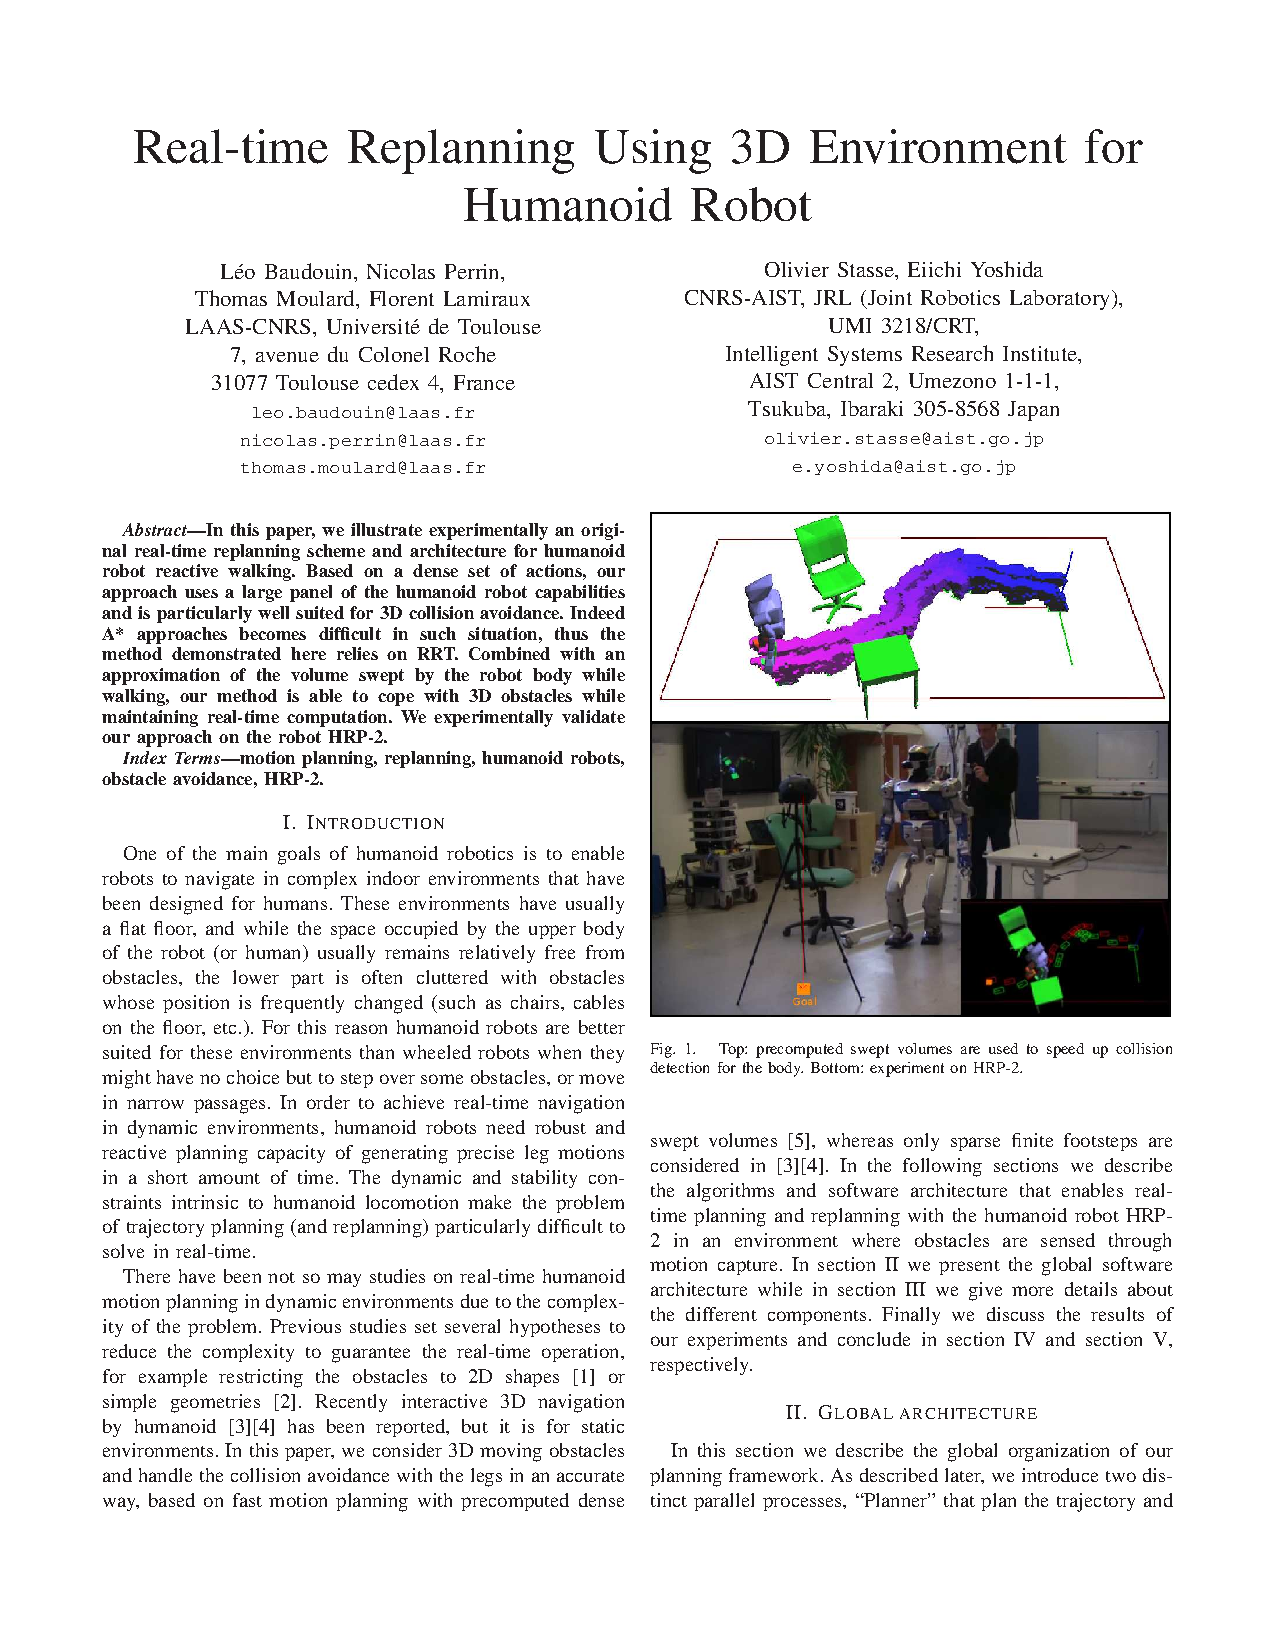
\includepdf[page=2]{humanoids11-lbaudouin.pdf} 
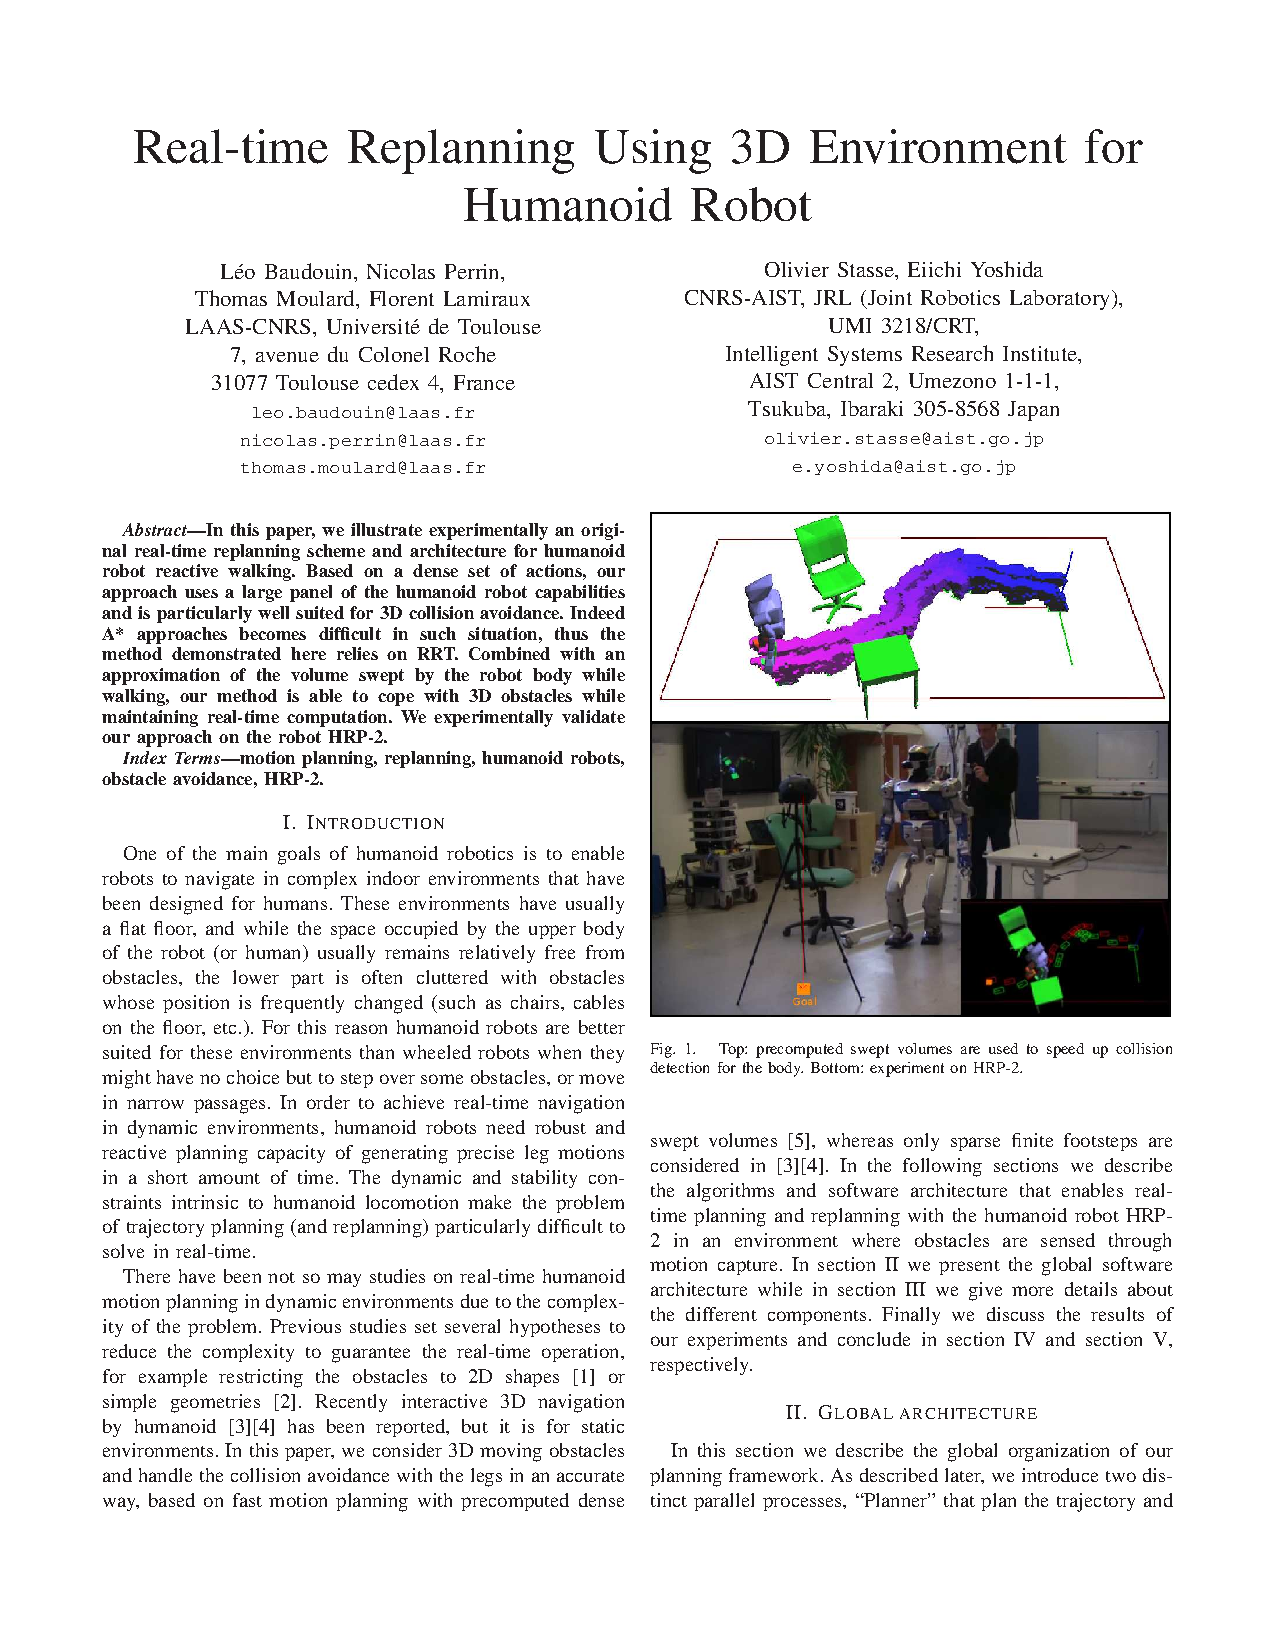
\includepdf[page=3]{humanoids11-lbaudouin.pdf} 
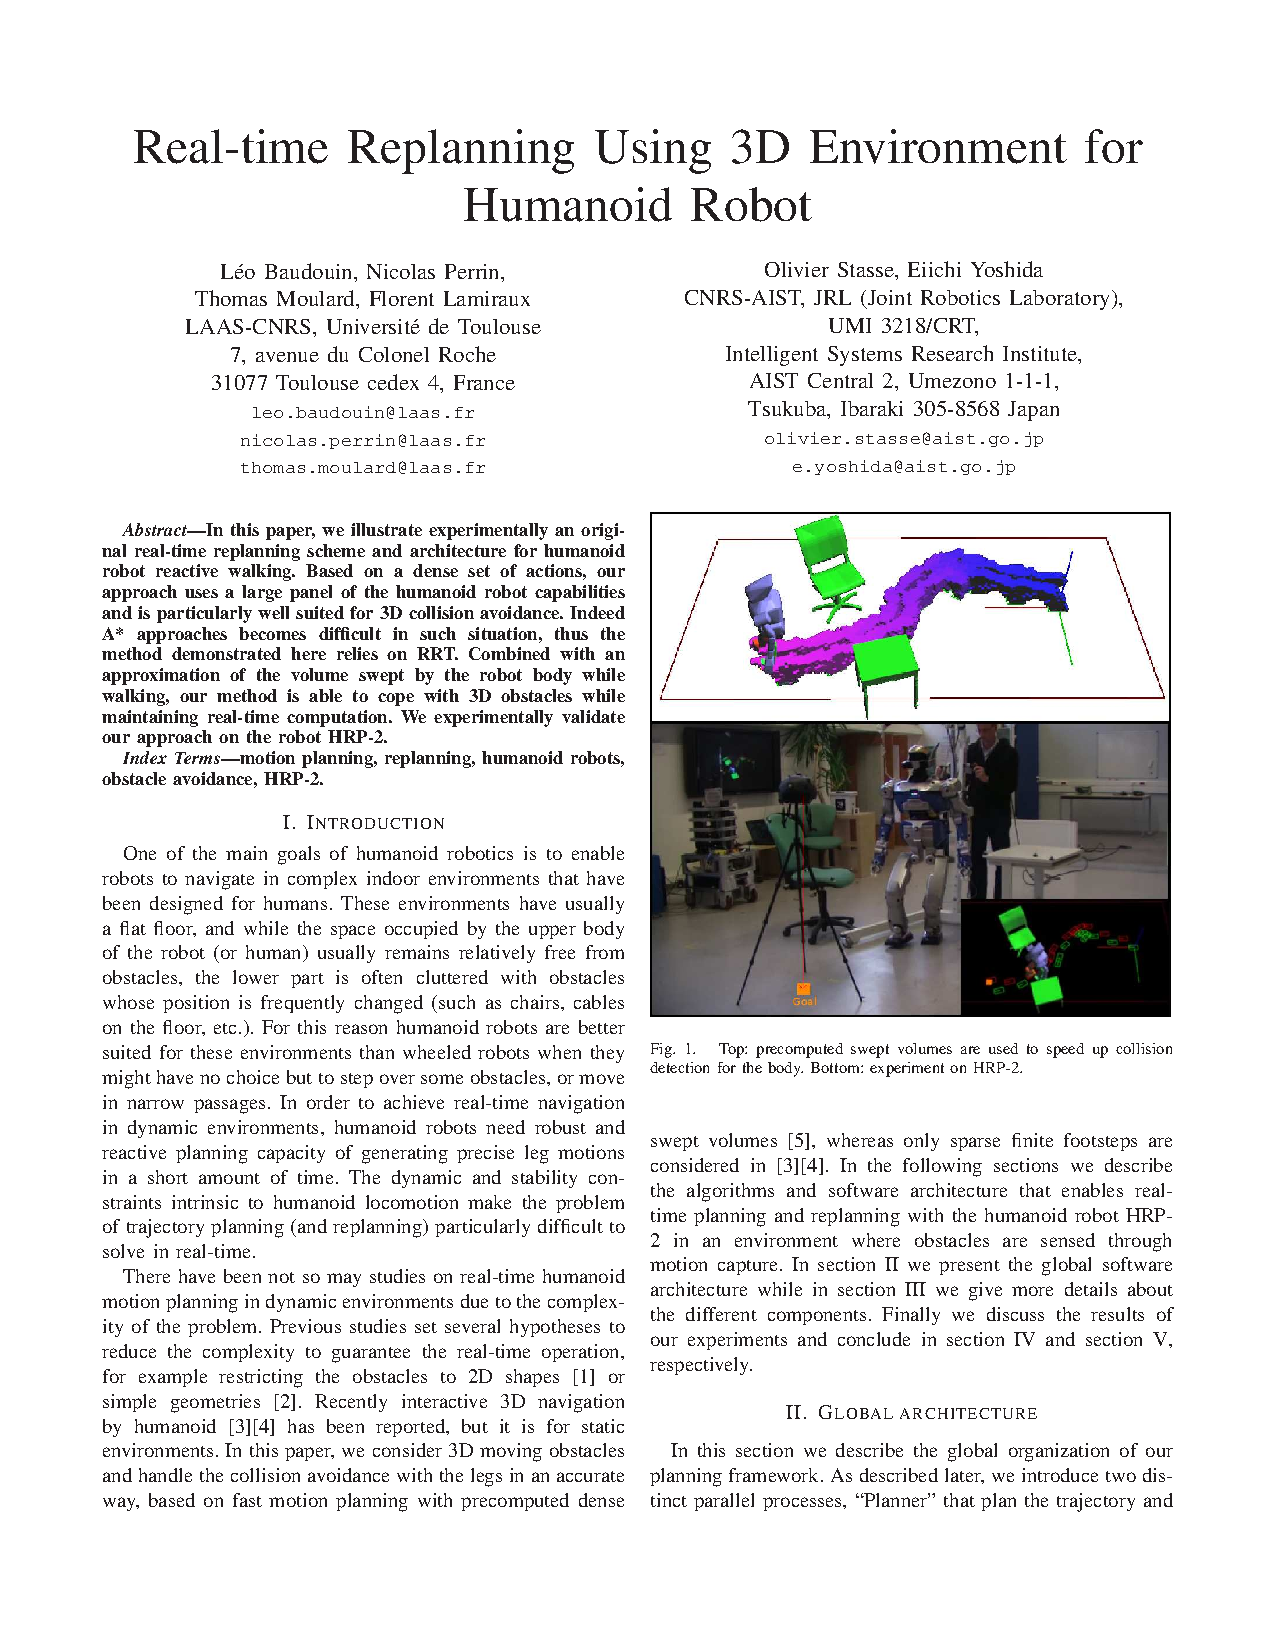
\includepdf[page=4]{humanoids11-lbaudouin.pdf} 
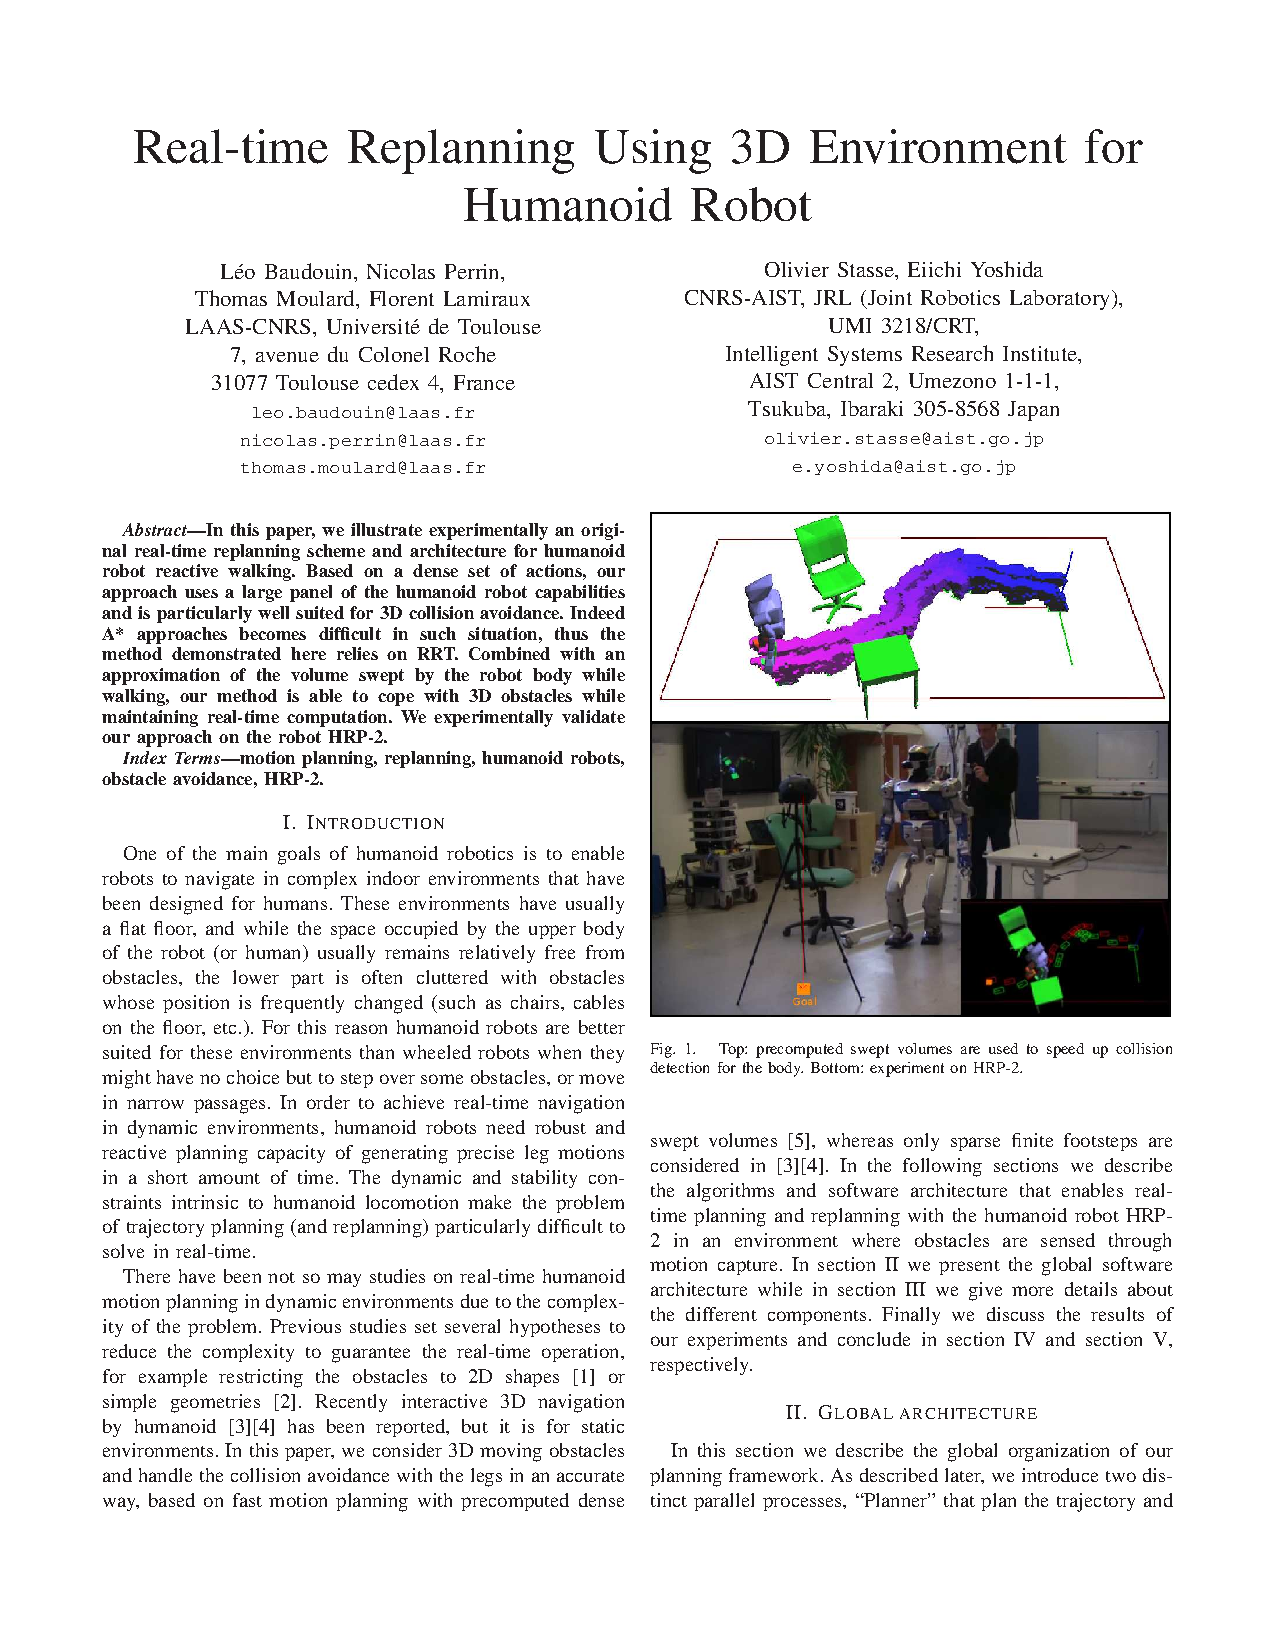
\includepdf[page=5]{humanoids11-lbaudouin.pdf} 
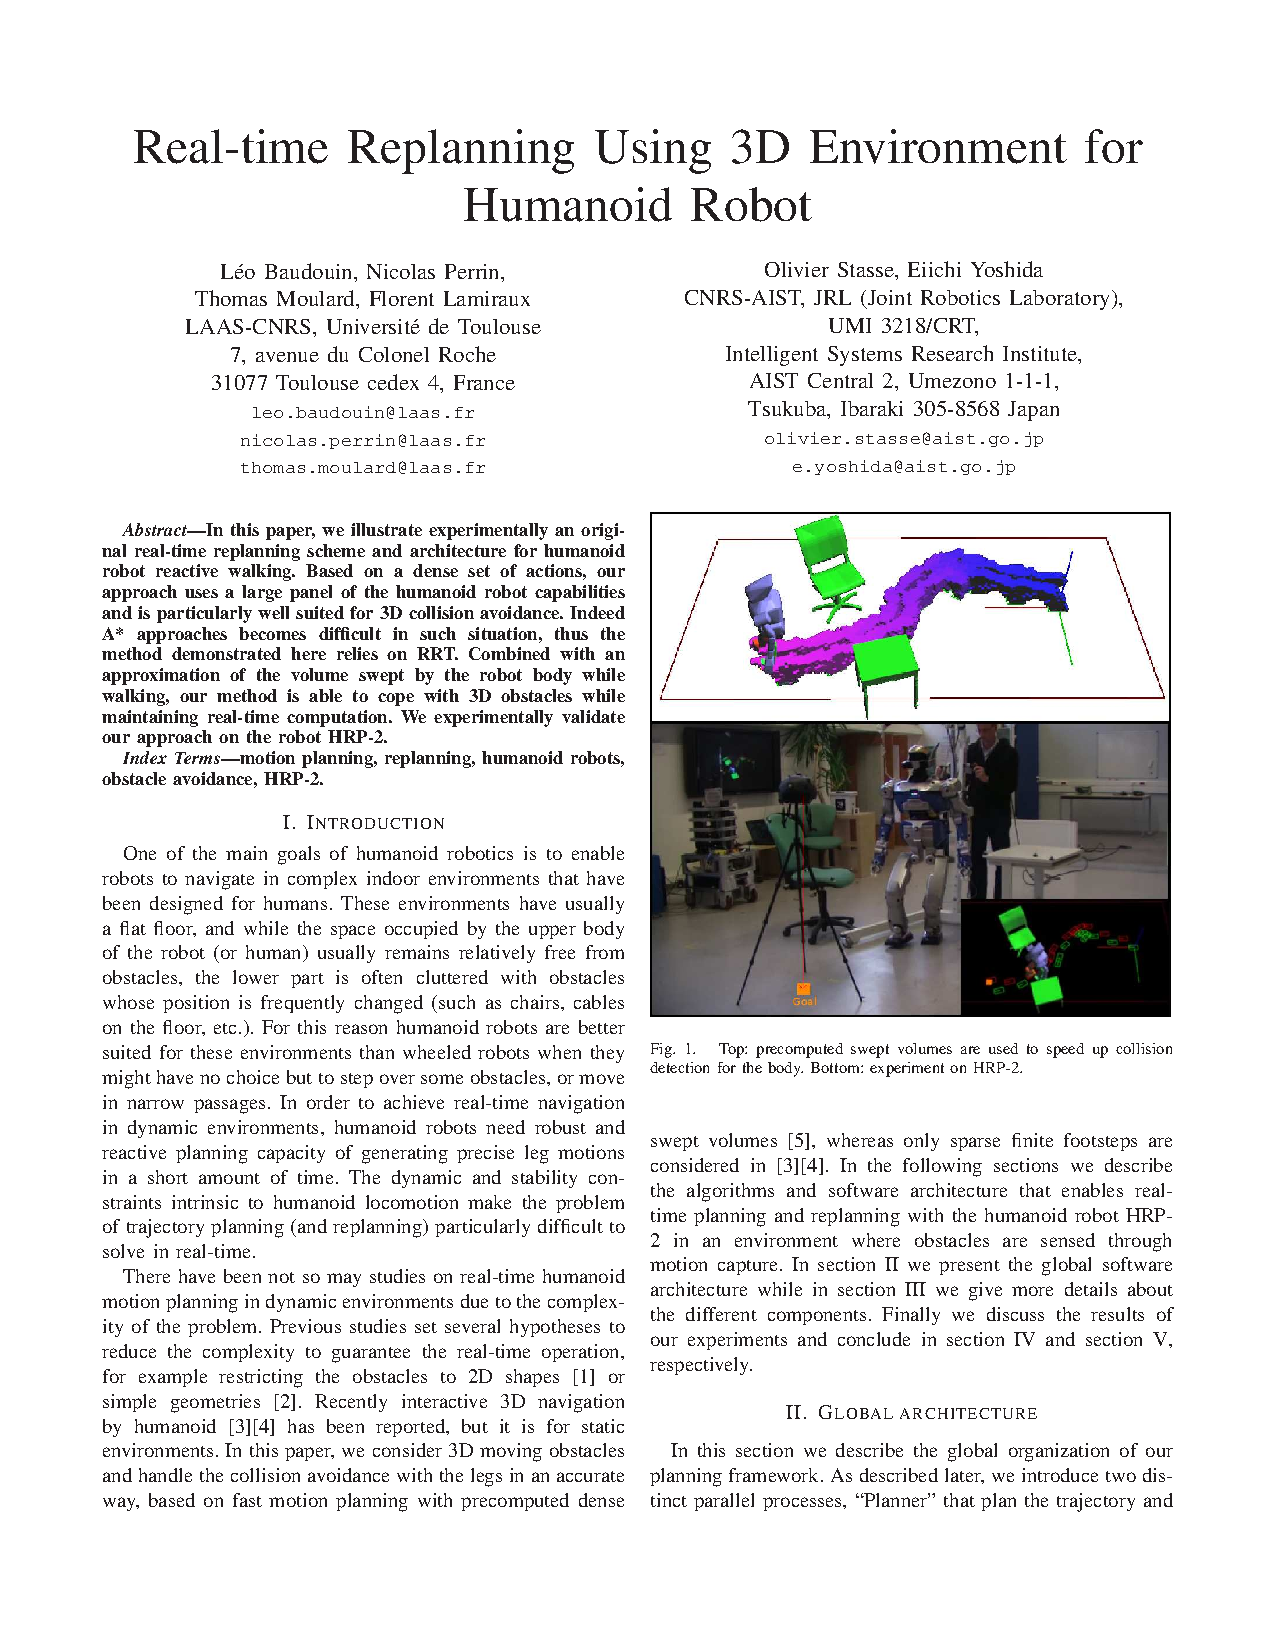
\includepdf[page=6]{humanoids11-lbaudouin.pdf} 


\section{Publication Transactions of Robotics 2011}

Publication pour Transactions of Robotics 2011.\\
\emph{Fast humanoid robot collision-free footstep planning
using swept volume approximations}\\
\nicolas, \olivier, \leo, \florent et \eiichi.

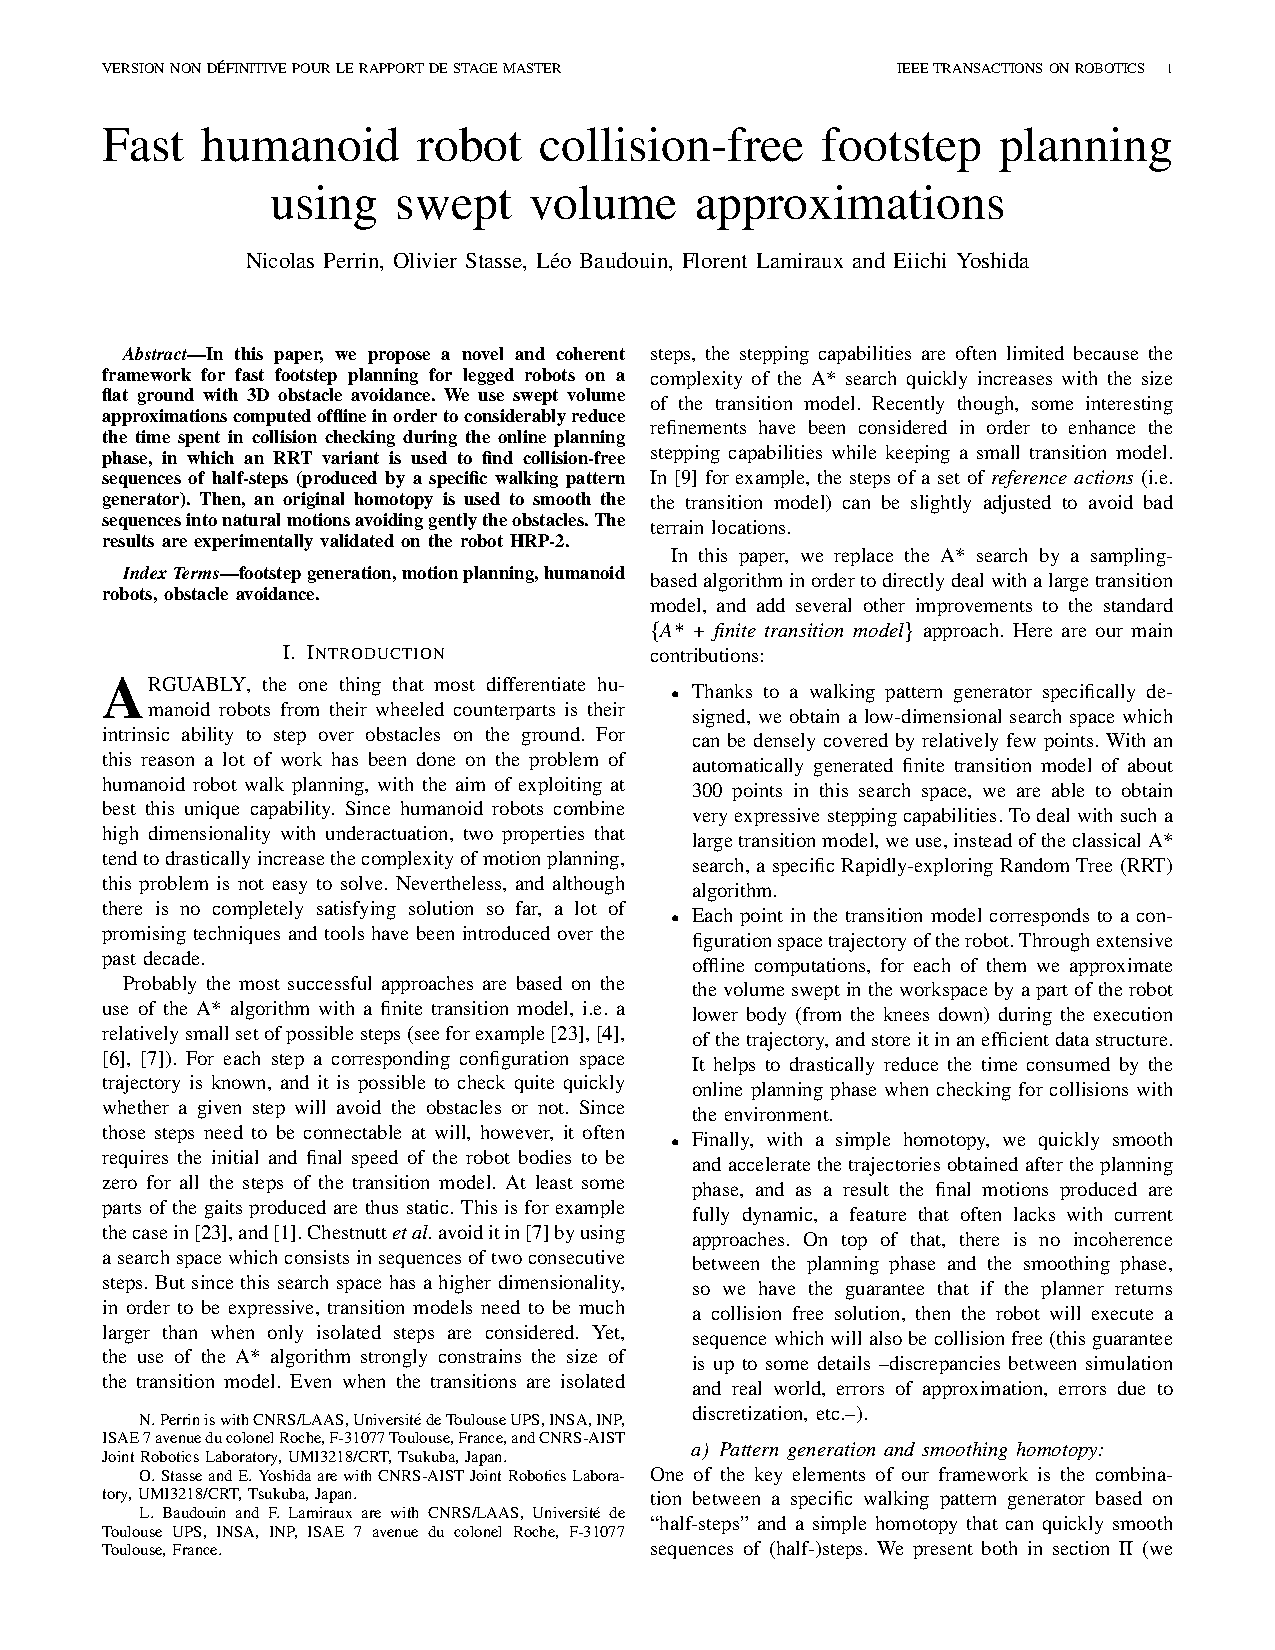
\includepdf[page=1]{troPaper.pdf}
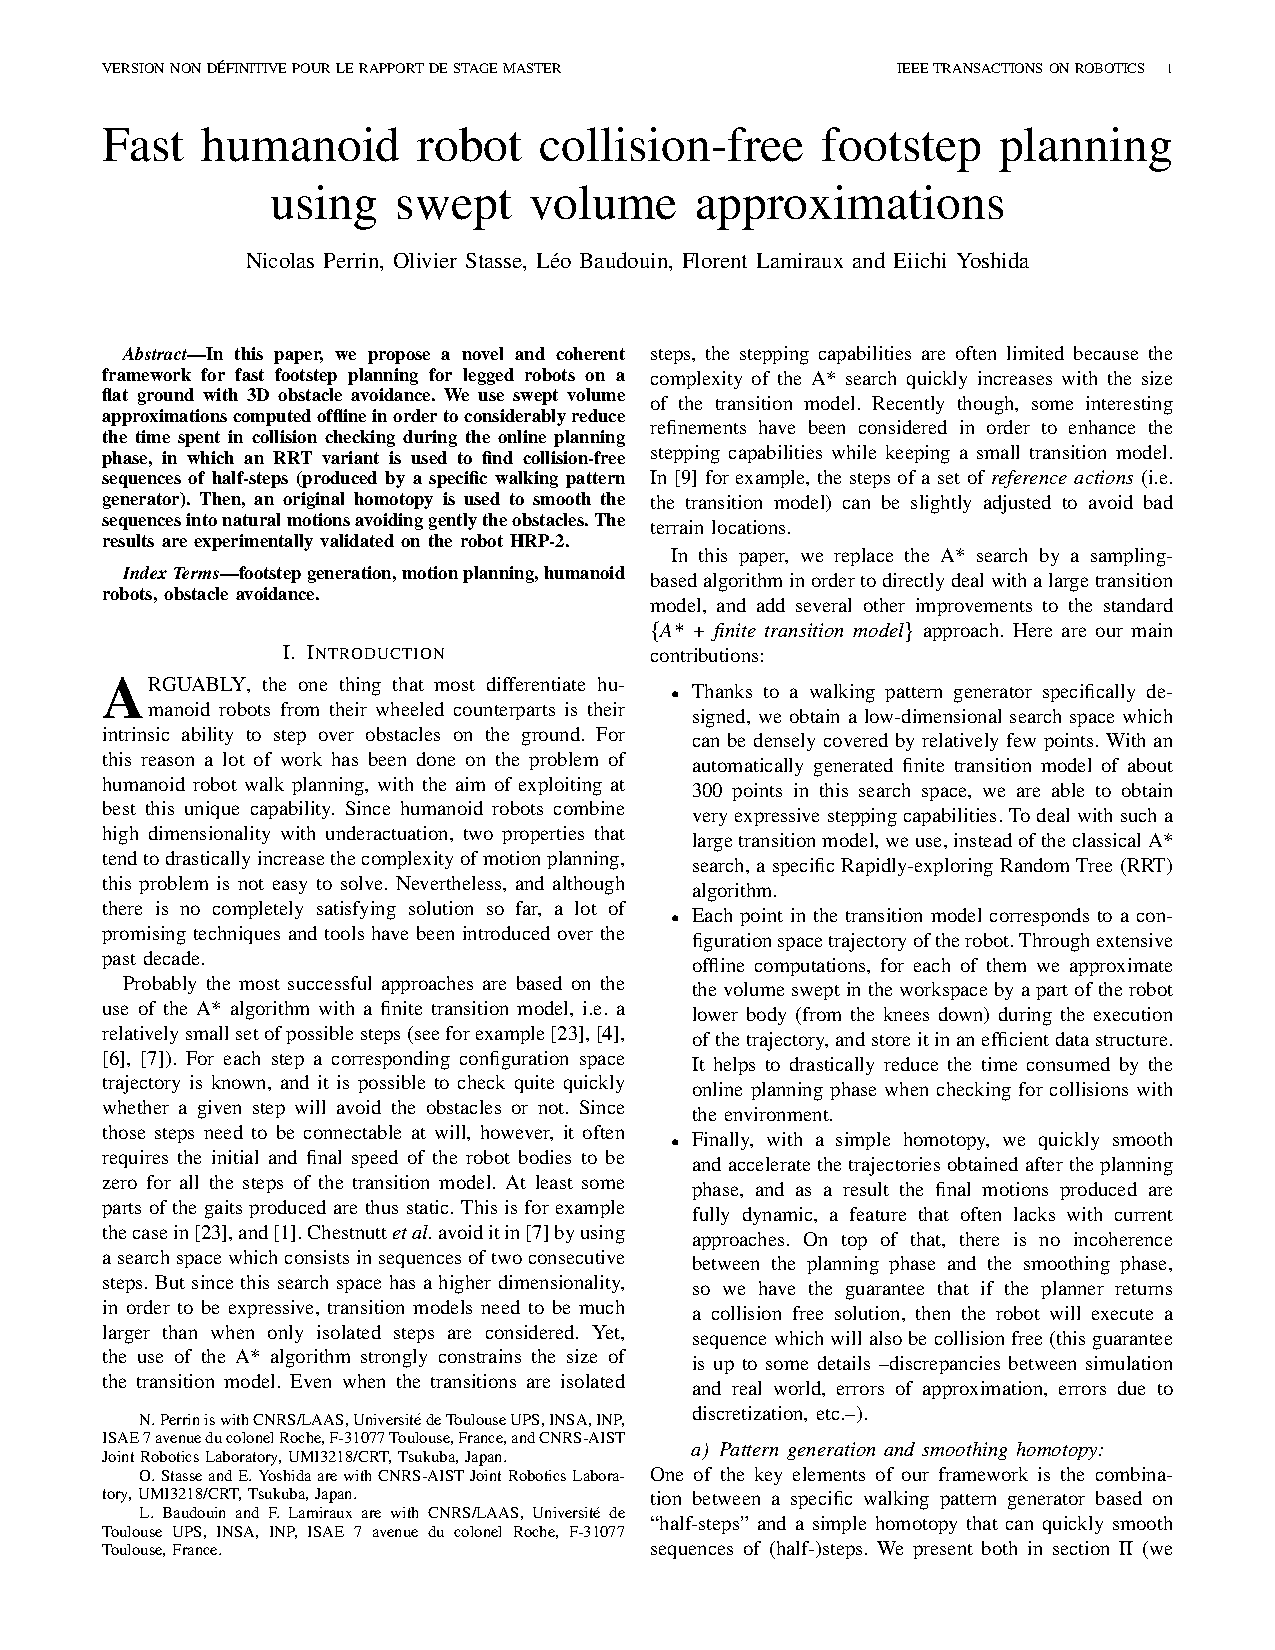
\includepdf[page=2]{troPaper.pdf}
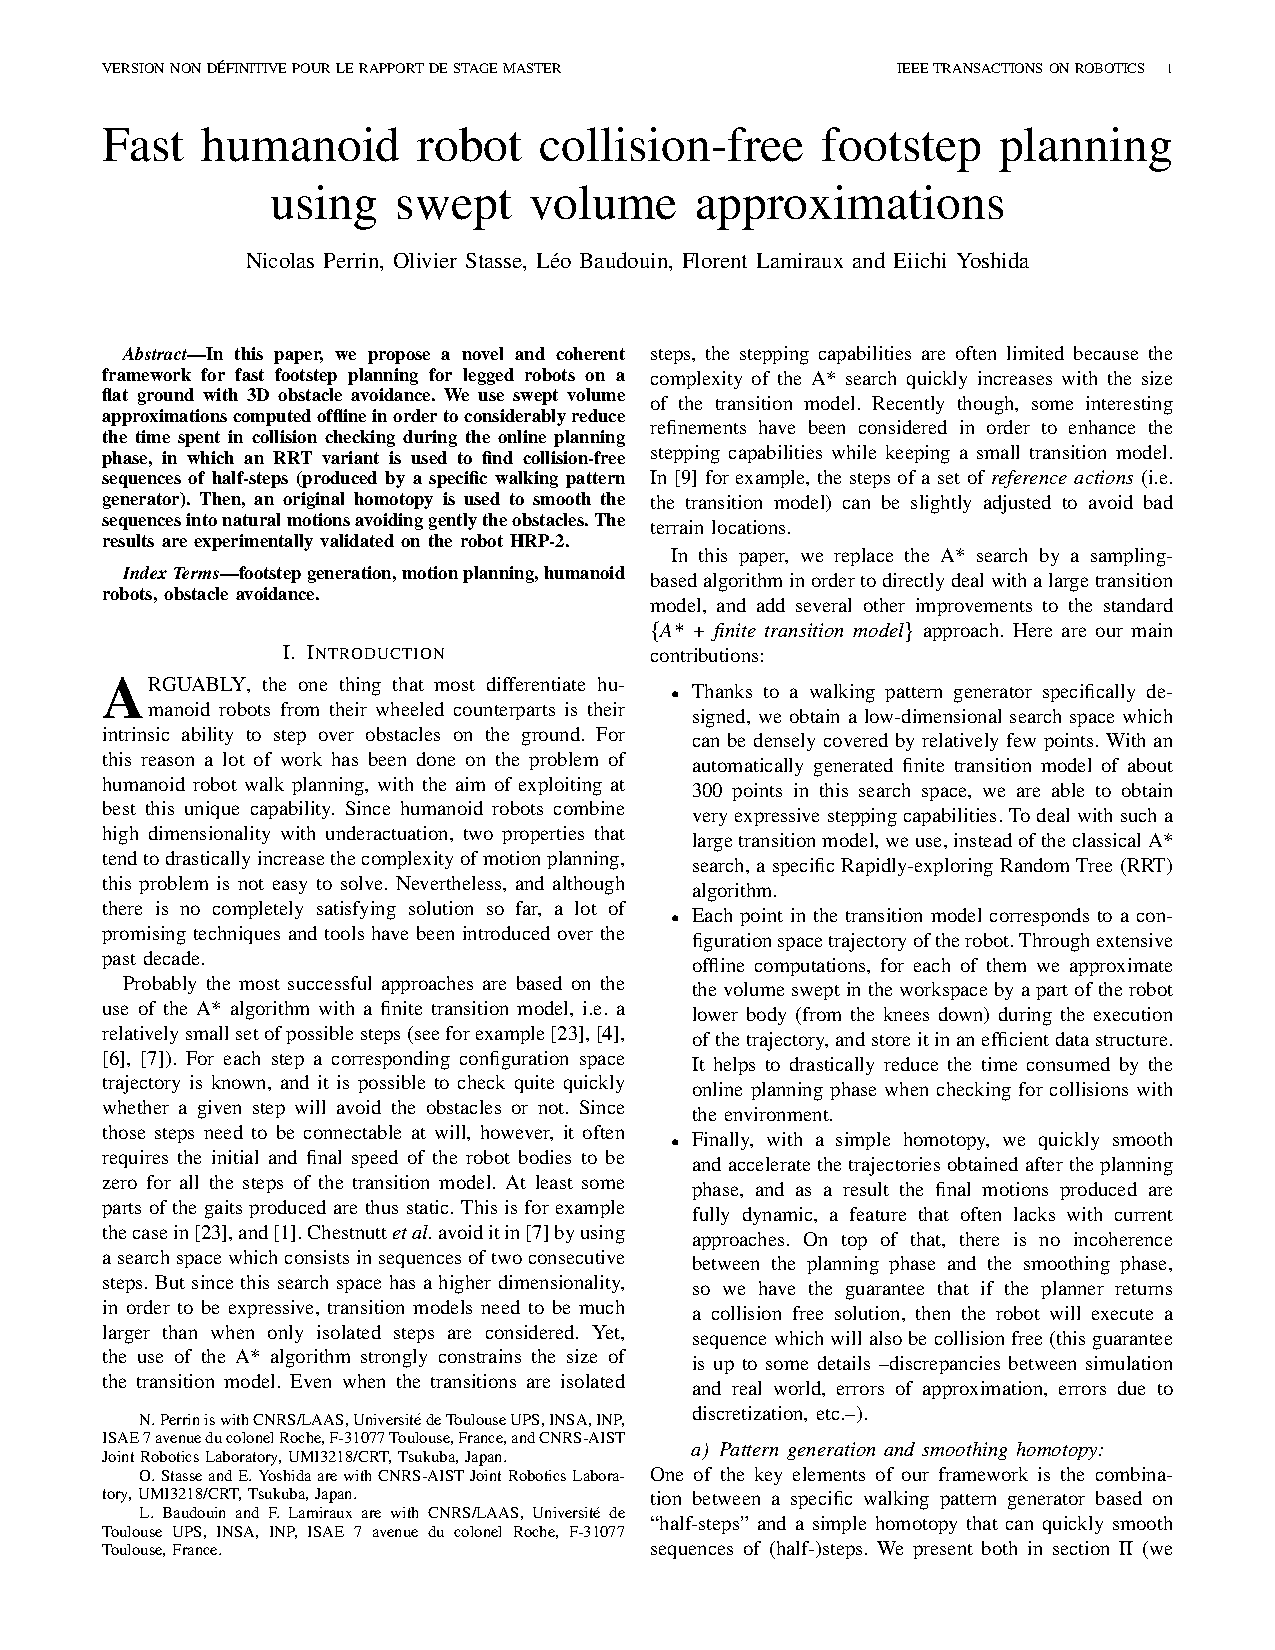
\includepdf[page=3]{troPaper.pdf}
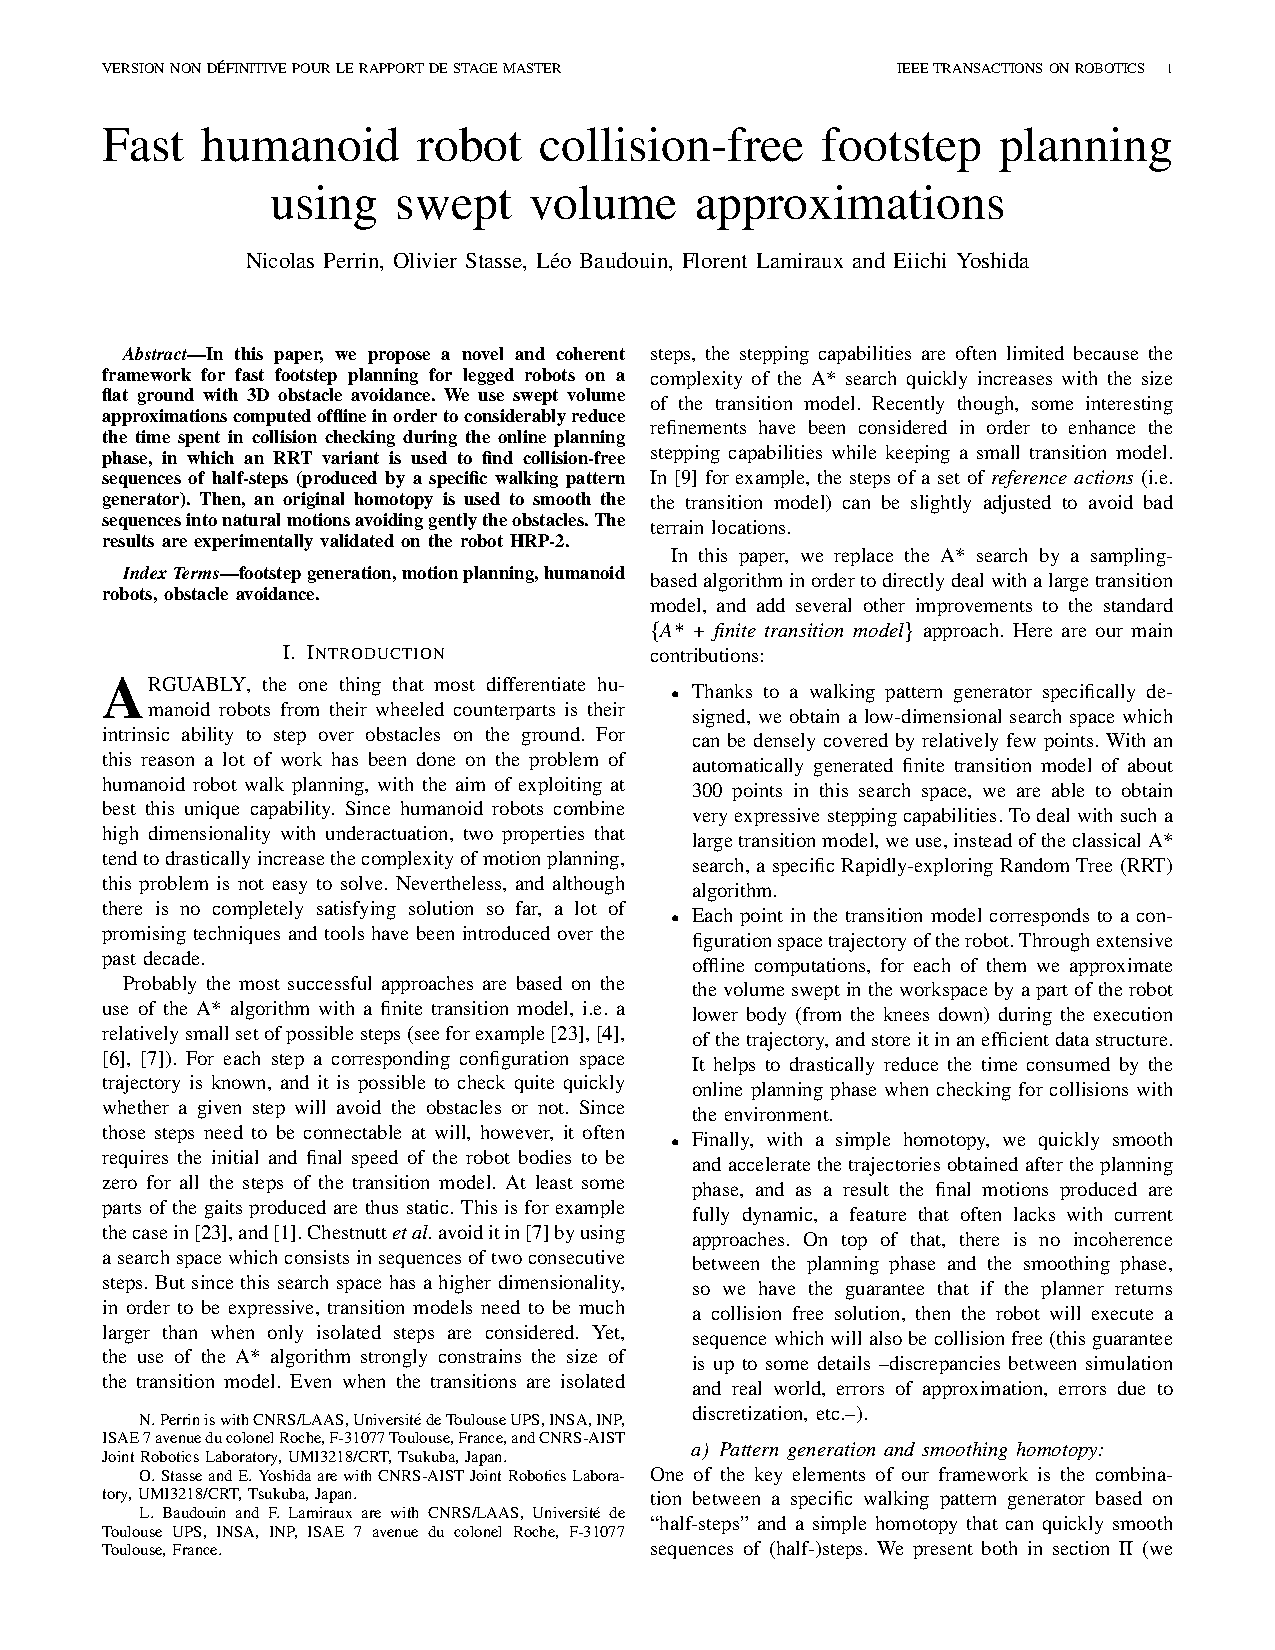
\includepdf[page=4]{troPaper.pdf}
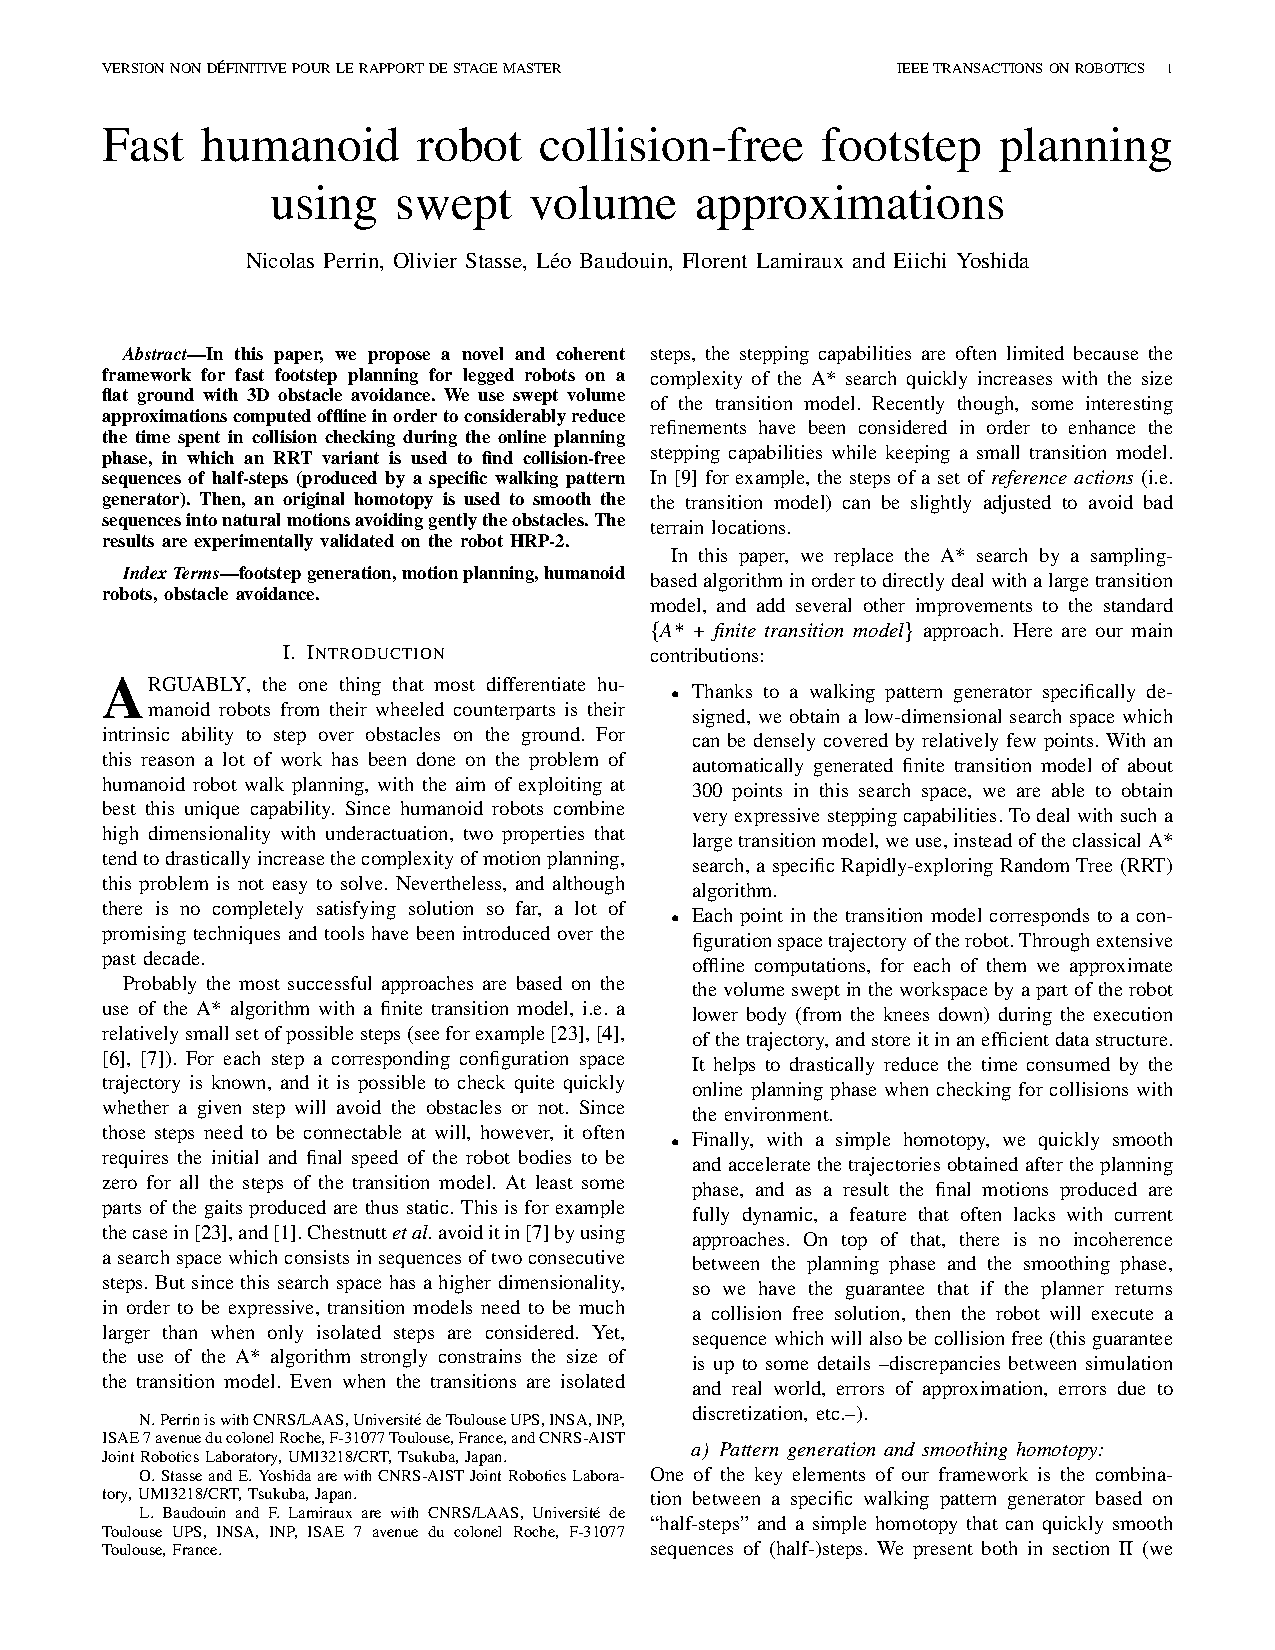
\includepdf[page=5]{troPaper.pdf}
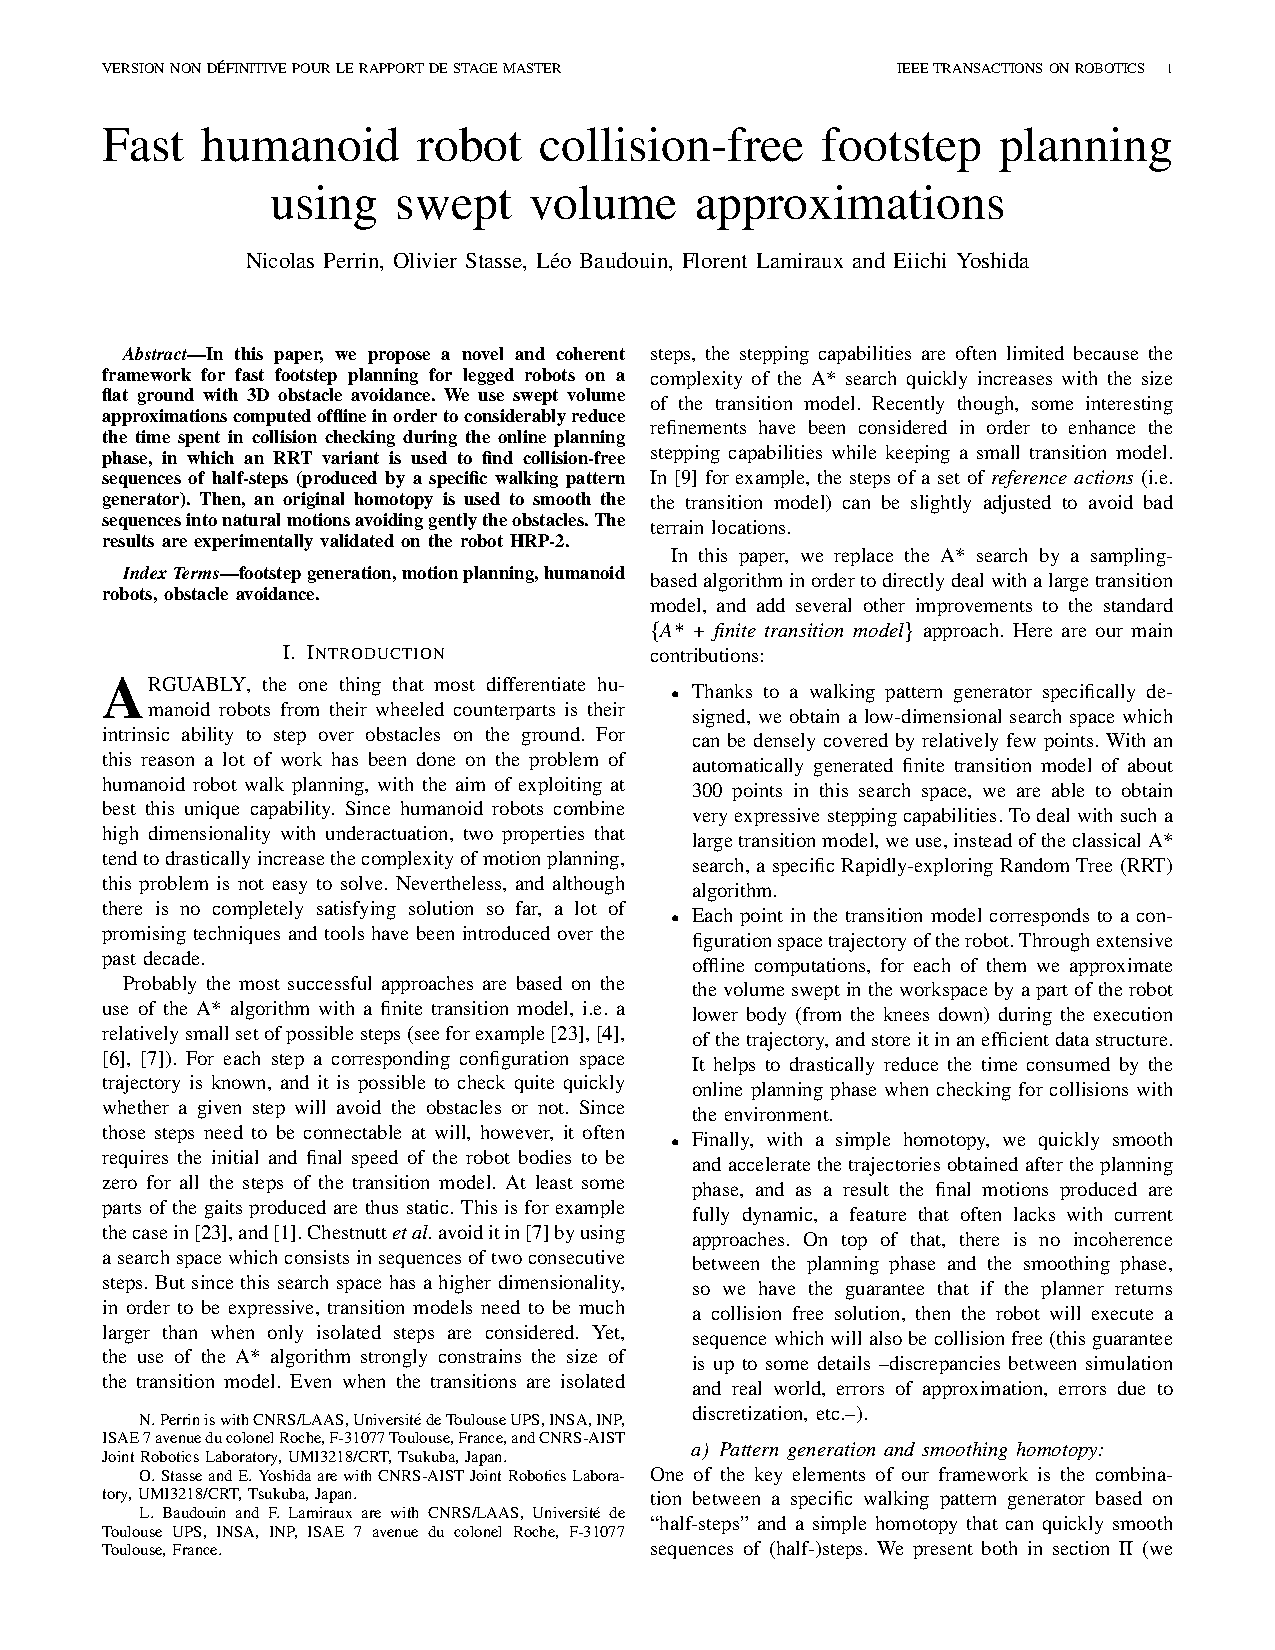
\includepdf[page=6]{troPaper.pdf}
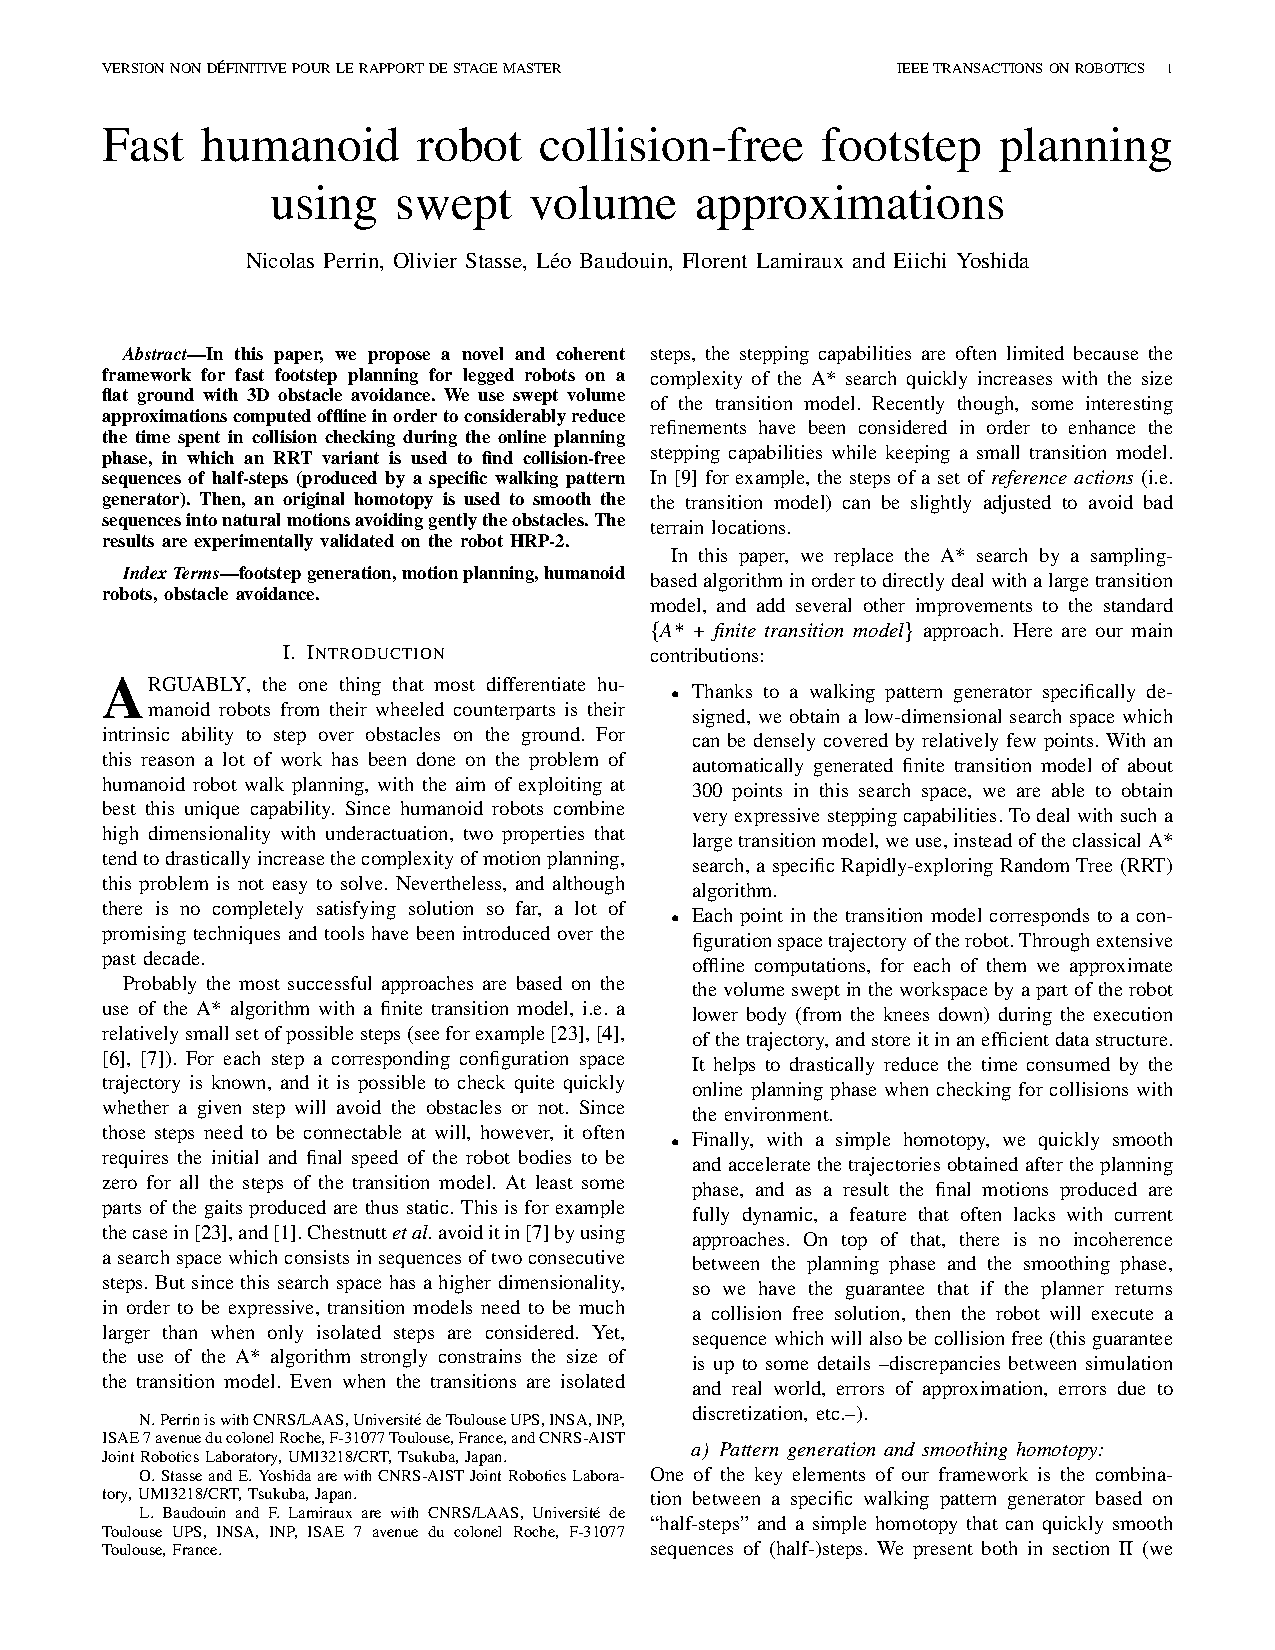
\includepdf[page=7]{troPaper.pdf}
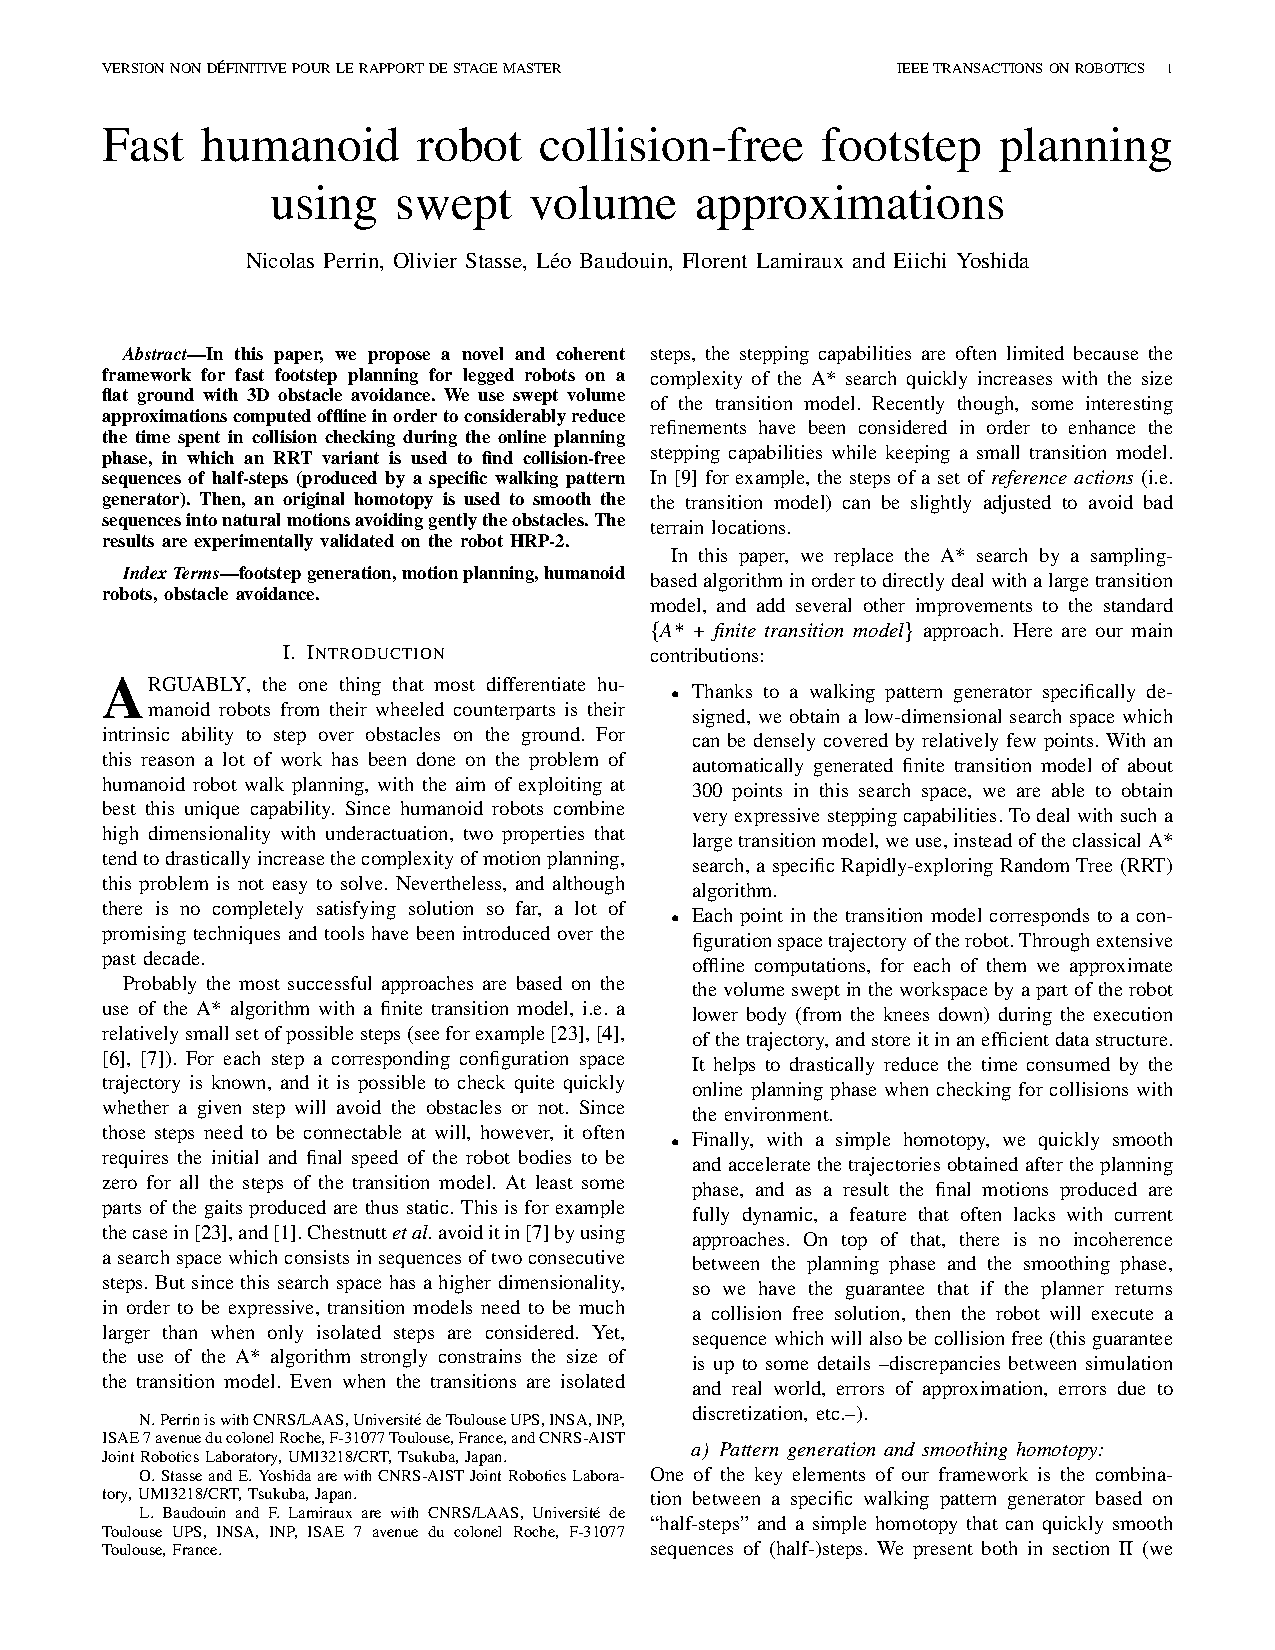
\includepdf[page=8]{troPaper.pdf}
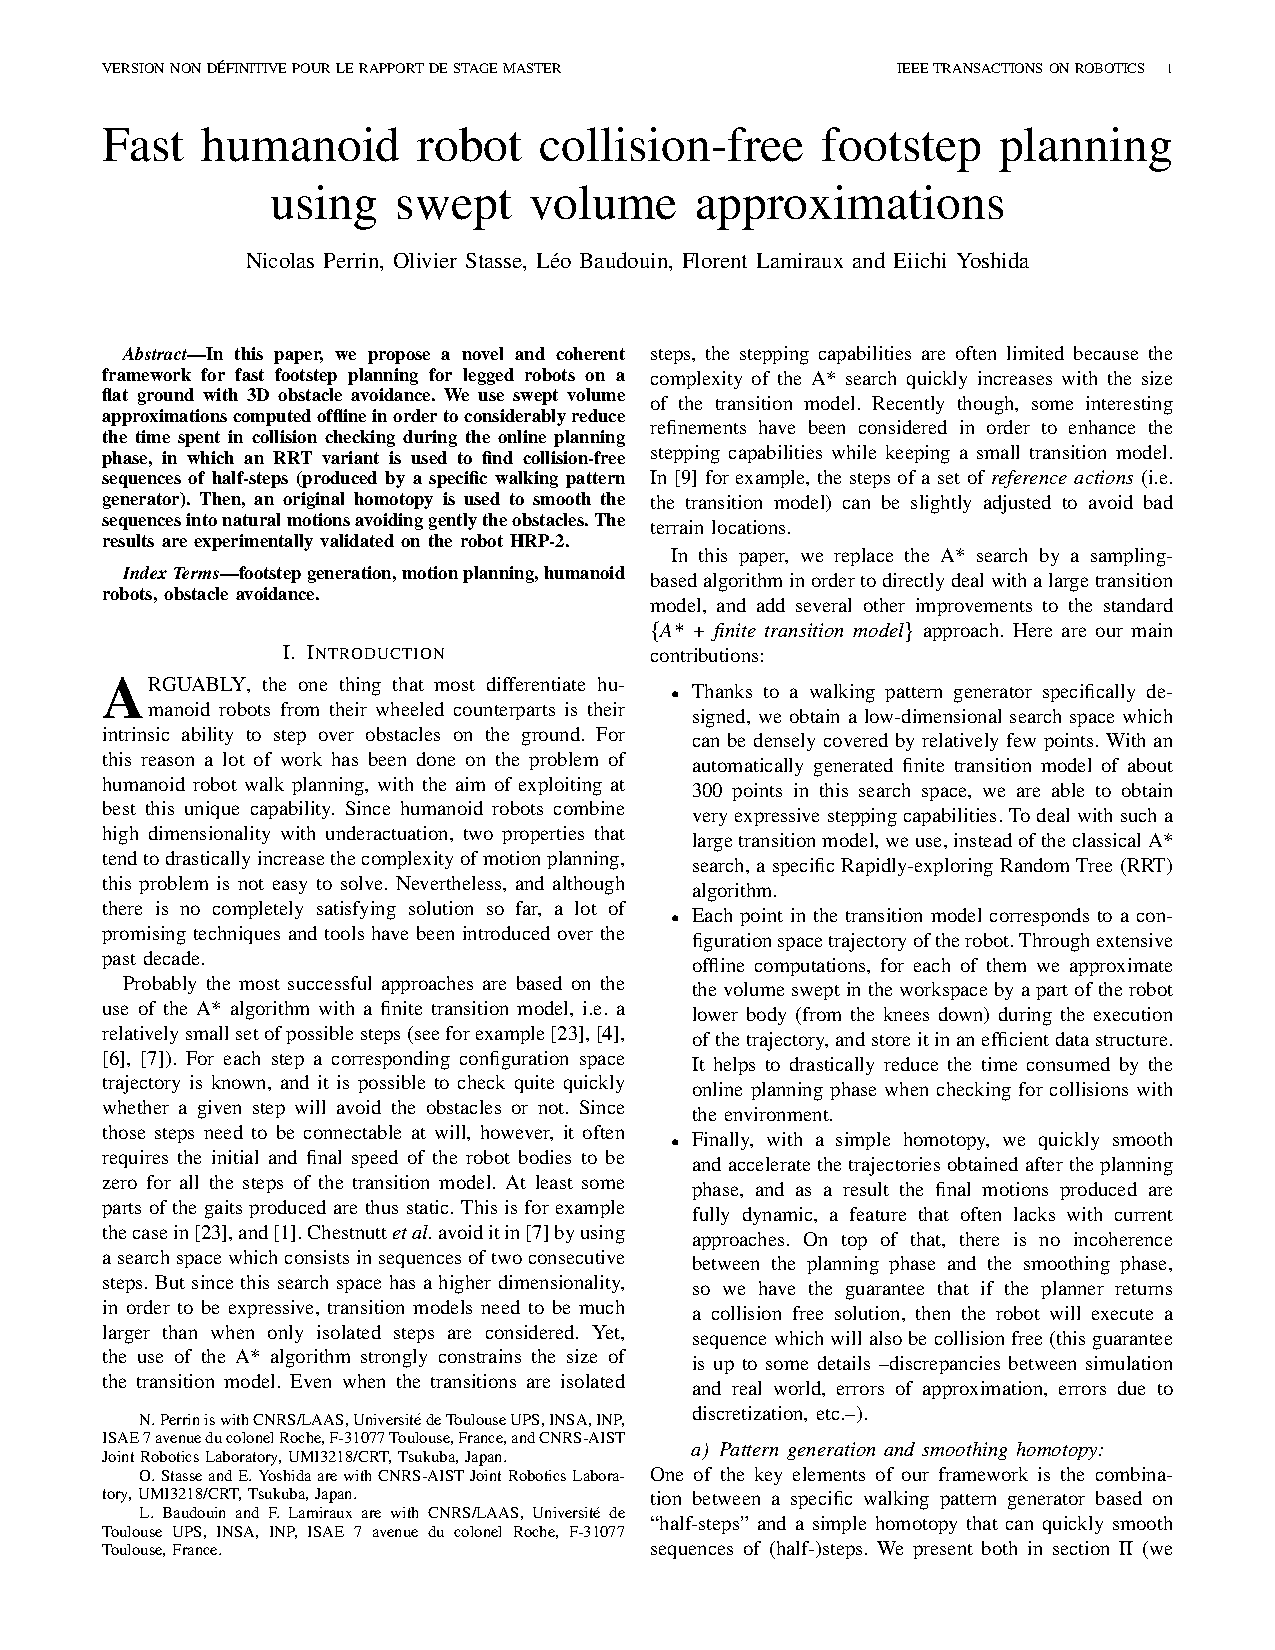
\includepdf[page=9]{troPaper.pdf}
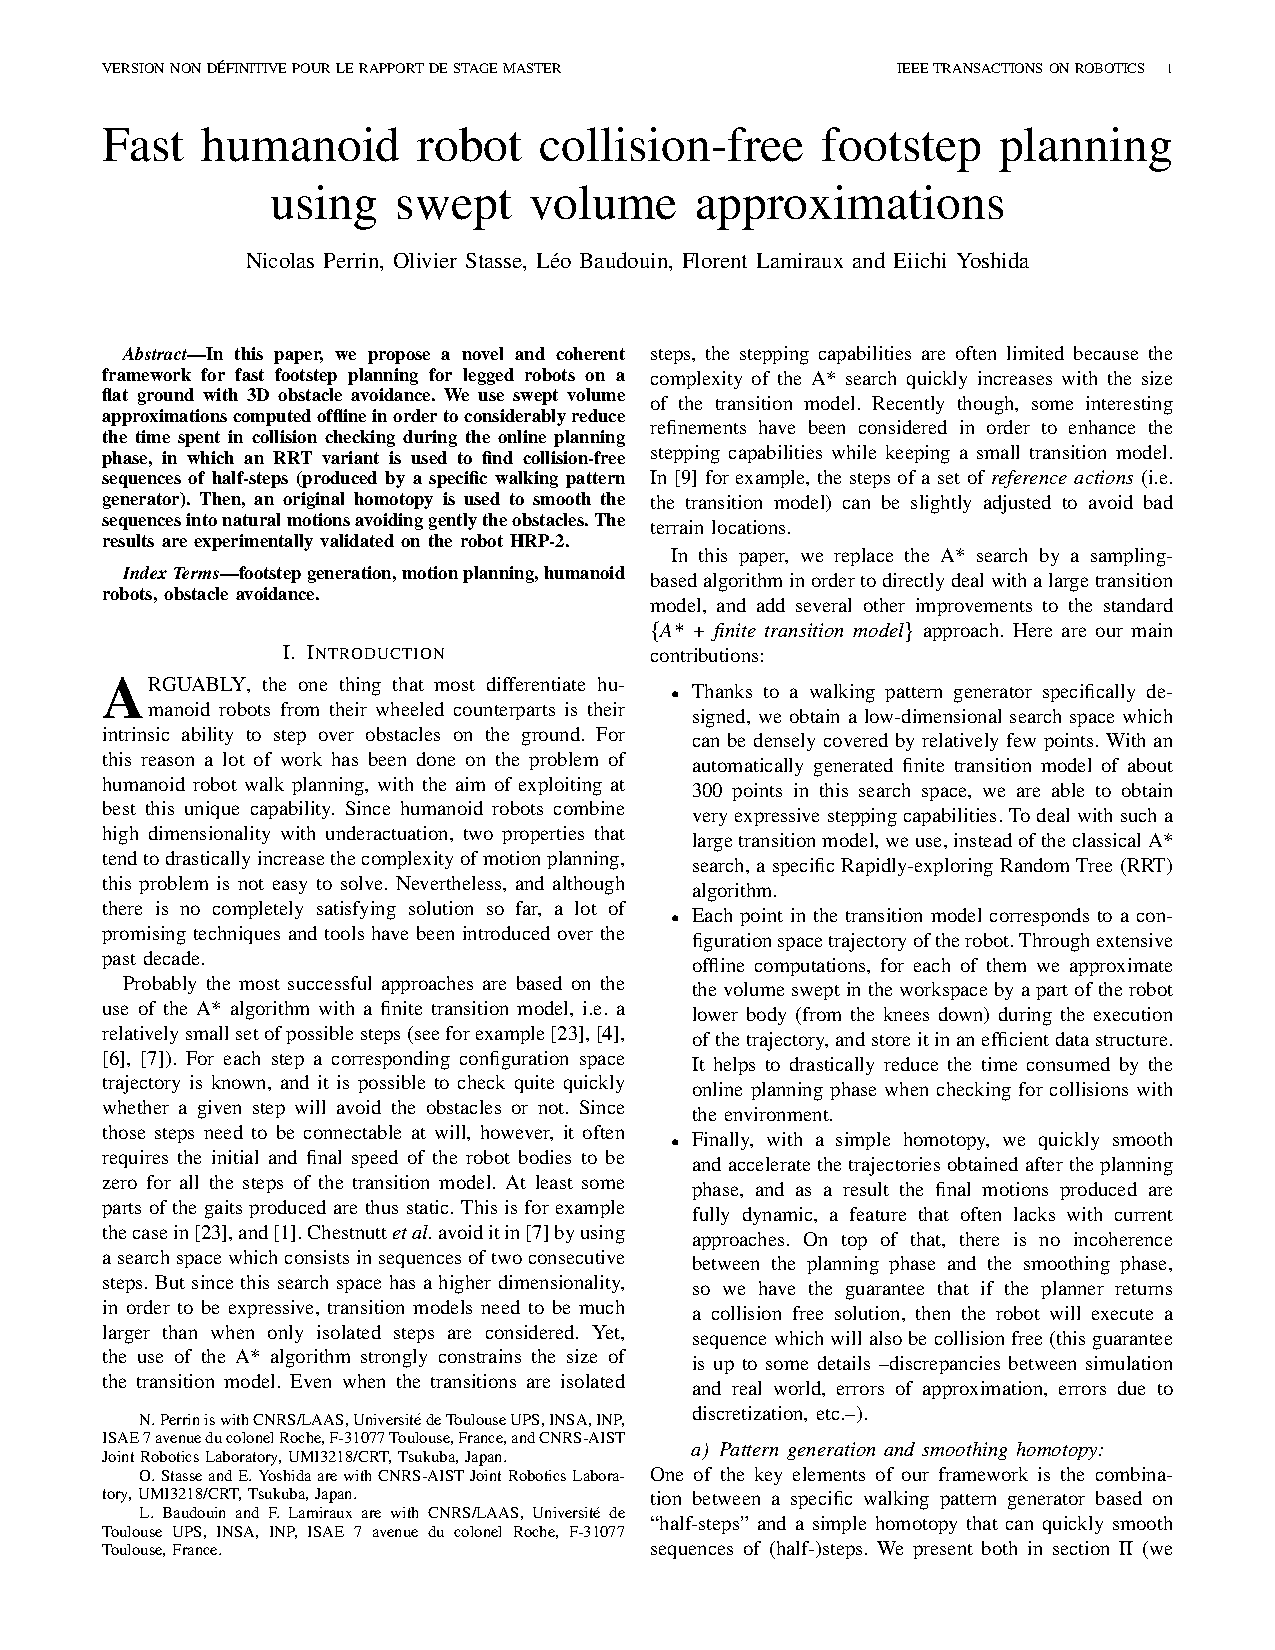
\includepdf[page=10]{troPaper.pdf}
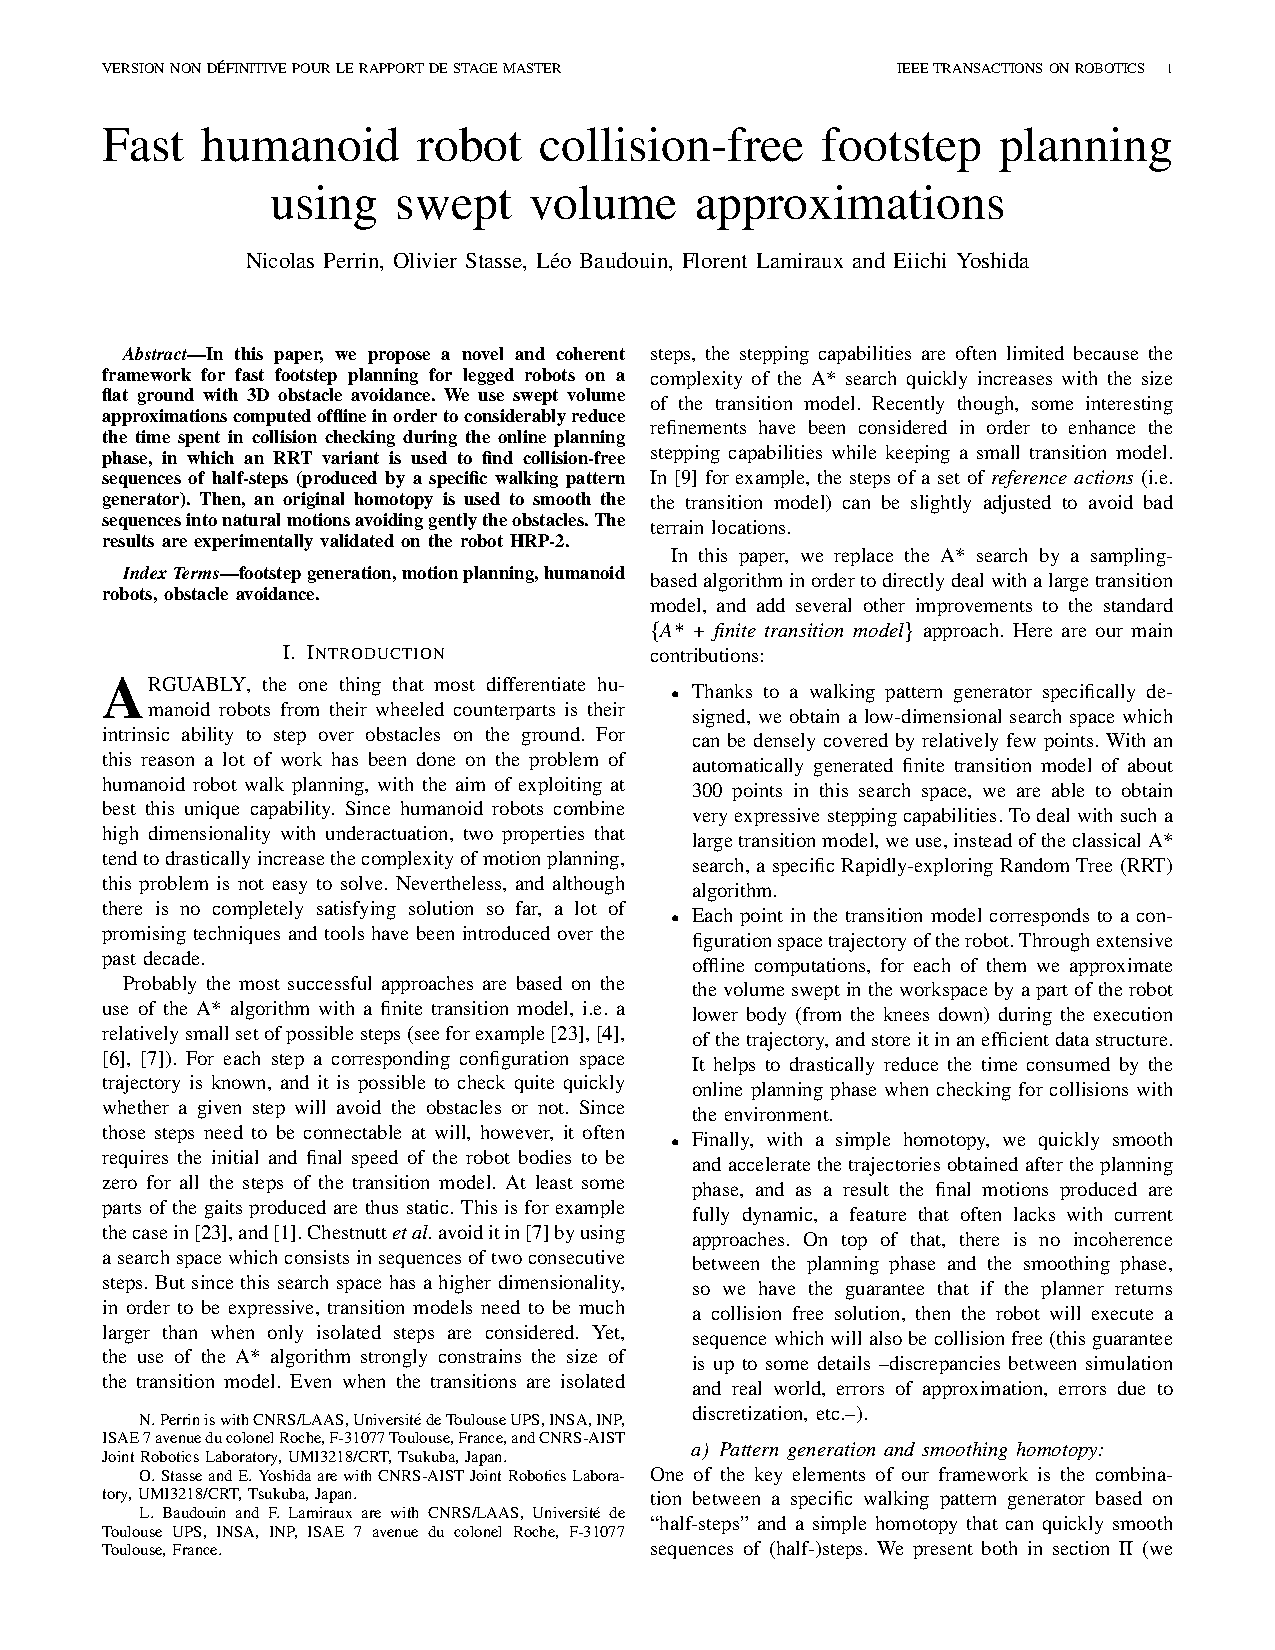
\includepdf[page=11]{troPaper.pdf}
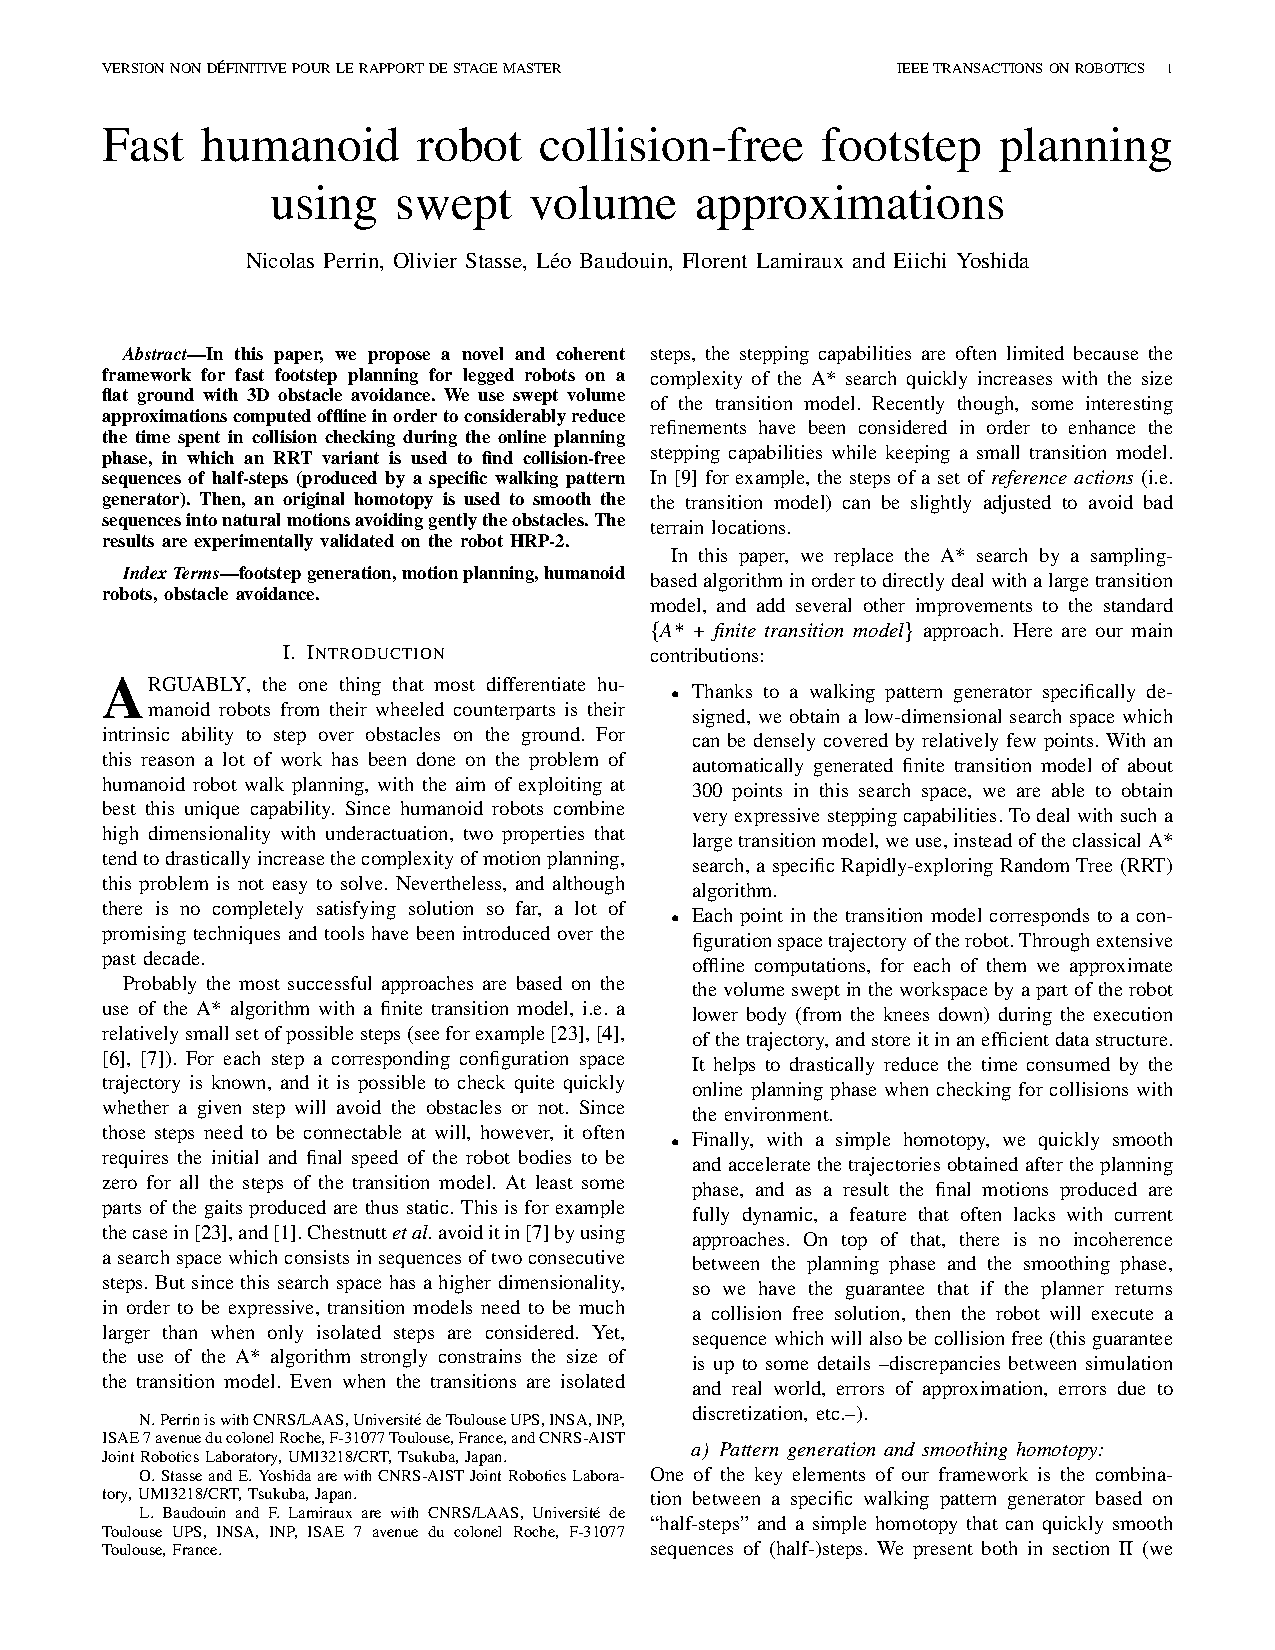
\includepdf[page=12]{troPaper.pdf}

\end{document}
